\documentclass{article}
\usepackage{graphicx}
\usepackage{ntheorem}[thmmarks]	% paquete de formateo de entornos matemáticos
\usepackage{listings}
\setlength{\parskip}{\baselineskip}%
\setlength{\parindent}{0pt}%
\theoremstyle{break}
\theoremheaderfont{\normalfont\bfseries}
\theorembodyfont{}
\theoremseparator{\vspace{0.2cm}}
\theorempreskip{\topsep}
\theorempostskip{\topsep}
\theoremindent0cm
\theoremnumbering{arabic}
\theoremsymbol{}
\theoremprework{\vspace{0.2cm}}
\theorempostwork{\vspace{0.2cm}}
    \newtheorem*{sprint}{Sprint}
    
\setlength{\parindent}{12pt}

\begin{document}
\graphicspath{{./fotos/}}


\section{Diseño y evolución de las clases principales del Modelo}
\subsection{Diseño del tablero}
Toda la lógica que implementa el concepto del tablero queda reflejada a lo largo de todo el proyecto en la clase Board.
\subsubsection{Sprint 1}
La clase Board es un simple contenedor de cubos, organizados en forma de matriz.
No tiene interacción con otros objetos del modelo.
\subsubsection{Sprint 2}
Ahora la clase Board tiene la funcionalidad de actualizarse a sí mismo una vez se coloca un nuevo cubo, funcionalidad que antes estaba delegada a la clase Game.
\subsubsection{Sprint 3}
A partir de este Sprint los tableros tienen forma (es decir, la forma no es necesariamente siempre cuadrada) y tamaño elegido por los usuarios. A parte, Board tiene una representación en forma de String y de JSONObject, a través de los métodos toString() y report().
\subsubsection{Sprint 5}
Ahora, aparte de guardarse los cubos del tablero en forma de matriz, se guardan en forma de lista por ser una representación de los datos muy conveniente en distintas partes del proyecto, entre otras, para la red.

\subsection{Diseño de los colores}

\subsection{Diseño de los cubos}

\subsection{Diseño del juego}
La clase fundamental del juego es la clase Game, la clase principal del modelo.
\subsubsection{Sprint 1}
La clase Game responde a ejecuciones del PlaceCubeCommand, colocando nuevos cubos en las casillas seleccionadas, actualizando el tablero, manejando los turnos de los jugadores y actualizando sus puntos.
\subsubsection{Sprint 2}
A partir de este momento, Game no se encarga de actualizar el tablero y las puntuaciones de los jugadores, sino de únicamente pasarle al tablero los cubos nuevos que tiene que insertar. El tablero, a partir de ese cubo, se actualiza a sí mismo, y los cambios de cubos actualizan las puntuaciones de los jugadores.
\subsubsection{Sprint 3}
Game tiene su propia representación en forma de String y de JSONObjet, a través de los métodos toString() y report().
\subsubsection{Sprint 4}
A partir de este sprint, Game pasa a ser una clase abstracta y se pasa a tener dos modos de juego, el clásico (jugadores individuales) y el modo por equipos, que son implementados por las clases herederas de Game: GameClassic y GameTeams.
También se implementa el patrón MVC, por lo que Game (modelo) pasa a tener una lista de observadores y métodos para el envío de notificaciones a estos.
\subsubsection{Sprint 5}
Game se adapta con ciertos cambios y nuevos métodos para soportar el juego en línea.
\subsubsection{Sprint 6}
En este momento Game sufre su mayor refactorización. Esta clase pasa a extender de la clase Thread, de forma que ya no funciona ejecutando comandos en el mismo momento de su creación, sino que estos de ponen en espera y Game, que está en todo momento funcionando y comprobando si hay nuevas peticiones puestas en espera, las ejecuta cuando puede. Esto nos permite evitar problemas de desbordamiento con el cálculo de jugadas por parte de las inteligencias artificiales, aparte de permitir el funcionamiento esperado de la vista sin comprometer su rendimiento.
Aparte, Game deja de llevar a cabo el manejo de turnos y se delega esa responsabilidad a la clase TurnManager, que es invocada tras cada jugada para que ejecute (si procede) el siguiente turno.

\subsection{Diseño de los jugadores}

\subsection{Diseño de los equipos}

\subsection{Diseño del gestor de turnos}

\subsection{Diseño de los estados del juego}

\subsection{Diseño de las replays}

\subsection{Diseño de las Inteligencias Artificiales}
\subsubsection{Sprint 5}
Las estrategias son externas al modelo. El cómputo de movimientos a través de estas estrategias de hace a partir de la vista, a través de la clase PlayerView, que representa al Player en la vista y se encarga de ejecutar sus acciones. Por razones de encapsulación, las estrategias no tienen acceso al modelo y realizan sus cálculos a través de GameStates.
\subsubsection{Sprint 6}
Las estrategias ahora forman parte del modelo, siendo atributo de aquellos Players controlados por la máquina. Como en este punto el manejo de turnos se lleva a cabo por la clase TurnManager y el modelo funciona en su propia hebra, la clase PlayerView desaparece del proyecto y son los propios players quienes ejecutan las estrategias, que a nivel abstracto resulta mucho más intuitivo. Por la hebra del modelo, cuando las estrategias terminan de calcular el siguiente movimiento, este no se ejecuta en ese mismo instante, sino que se deja en espera en el modelo hasta que este pueda ejecutarlo.


\section{Diseño del Controlador}


\section{Diseño de la Vista de GUI}

\subsection{Diseño del menú principal y pantallas pre-juego}

\subsection{Diseño de la pantalla de juego}


\section{Diseño de la Vista de Consola}

\subsection{Diseño del menú principal y pantallas pre-juego}

\subsection{Diseño de la pantalla de juego}


\section{Diseño de la red}

\subsection{Diseño del servidor}

\subsection{Diseño de los clientes}


\section{Diseño y evolución de las Historias de Usuario}

\subsection{Como usuario quiero poder jugar a Rolit con una interfaz agradable}

\subsubsection{JUANDI - Como usuario, me gustaría que se pudiesen personalizar los colores con los que jugamos cada jugador porque hace más visual el juego.}

\subsection{Como usuario, me gustaría que tenga una interfaz gráfica amable porque hace más fácil jugar.}
\begin{sprint}[1 JUANDI]

\end{sprint}

\begin{sprint}[2 JUANDI]

\end{sprint}

\begin{sprint}[3 JUANDI]

\end{sprint}

\begin{sprint}[4]
\textbf{Console - JUANDI}

aaaaa

\textbf{GUI}

En este sprint se desarrolló una primera versión de la interfaz gráfica, lo cual involucra a un gran número de clases y métodos. Iniciemos un recorrido por cada uno de los componentes visuales explicando su finalidad

\underline{CeldaGUI}
\begin{center}

\includegraphics[scale=0.5]{yellowCube.png}

\includegraphics[scale=0.5]{emptyCell.png}
\end{center}

Esta clase representa cada una de las posiciones del tablero y puede ser vacía o tener un cubo. La mayor parte de funciones de esta clase  tienen como objetivo cambiar el color del cubo que representa cada celda.

\underline{BoardGUI}
\begin{center}
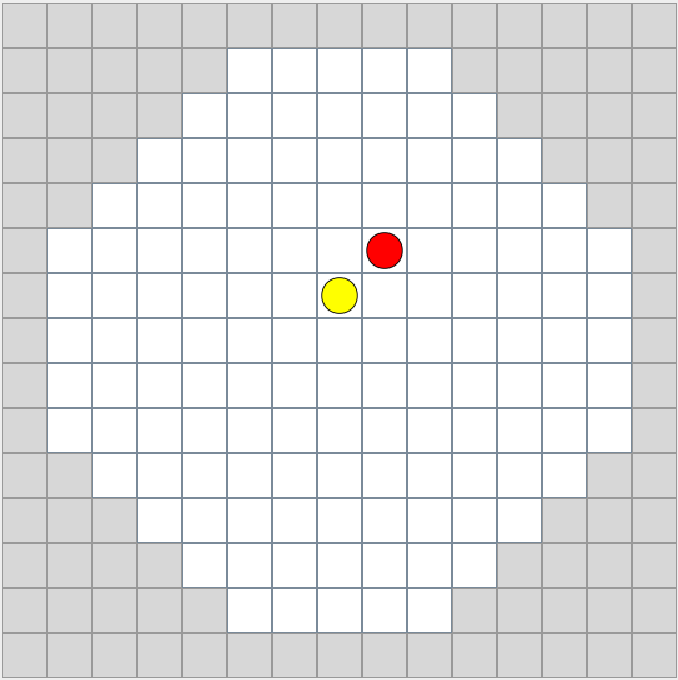
\includegraphics[scale=0.8]{board-gui-cubos-sprint3.png}
\end{center}

La clase \textit{BoardGUI} extiende de \textit{JPanel} y es la encargada de visualizar el tablero de la partida. Se puede apreciar que el tablero está formado por un conjunto de \textit{CeldaGUI}.

\underline{ControlPanel}
\begin{center}

\includegraphics[scale=0.8]{control-panel-sprint3.png}
\end{center}

El \textit{ControlPanel} es una \textit{JToolBar} que cuenta con un botón para guardar partidas, que puede ser pulsado en cualquier momento durante la ejecución del juego.

\begin{center}

\includegraphics[scale=0.8]{control-panel-replay-sprint3.png}
\end{center}

En el caso de las \textit{replays}, en el \textit{ControlPanel} aparecen dos flechas para poder recorrer los estados.

\underline{TurnAndRankingBar}
\begin{center}

\includegraphics[scale=1]{turn-ranking-panel-sprint3.png}
\end{center}

Esta clase es un \textit{JPanel} se encarga de mostrar a los usuarios del turno del jugador actual, las puntuaciones de cada uno de los participantes y la modalidad de juego.

\underline{StatusBar}


\underline{CreateGameDialog}
\begin{center}
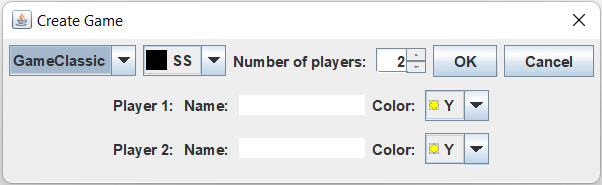
\includegraphics[scale=0.8]{create-game-sprint3.png}
\end{center}

Como su propio nombre indica, esta ventana extiende de \textit{JDialog} y tiene como objetivo poder configurar una partida desde cero, combinando todas las características posibles para crear un juego a gusto de los usuarios.

En esta pantalla el usuario elige el modo de juego para la partida (\textit{GameClassic} o \textit{GameTeams}), la forma y tamaño del tablero (cuadrado, círculo o rombo, pequeño, mediano o grande), el número de jugadores (entre 2 y 10, ambos inclusive) y el nombre y color de cada jugador.

En caso de seleccionarse el modo por equipos, el usuario introducirá el nombre de ambos equipos y el equipo al que pertenece cada jugador.

Una vez el usuario presiona el botón \textit{OK} se le lleva a la pantalla de juego.

Si el usuario presiona \textit{Cancel} se le lleva de vuelta a la pantalla principal.

\underline{LoadGameDialog}
\begin{center}
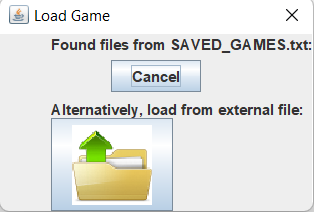
\includegraphics[scale=0.8]{load-dialog-sprint3.png}
\end{center}

En esta pantalla se muestra una lista con las partidas guardadas, de forma que si se elige una de estas partidas se cargará inmediatamente.

Aparece también debajo un botón de carga de ficheros que abre un  \textit{JFileChooser} por si se quiere cargar un juego que no esté incluido en la lista de partidas guardadas.

\underline{DeleteGameDialog}
\begin{center}
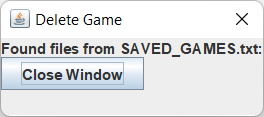
\includegraphics[scale=0.8]{delete-dialog-sprint3.png}
\end{center}

En esta pantalla se muestra la lista de partidas guardadas y un botón para confirmar el borrado. Con esto, si se selecciona una de las partidas guardadas y se presiona el botón inferior, la lista se elimina de la lista de partidas guardadas.

\underline{StatusBar}
\begin{center}

\includegraphics[scale=0.8]{status-bar-sprint3.png}
\end{center}

La \textit{StatusBar} es un \textit{JPanel} que se encarga de mostrar información relevante durante la partida, como mensajes de error o de confimación, otorgándole al usuario un feedback adecuado.

\underline{MainWindow}
\begin{center}
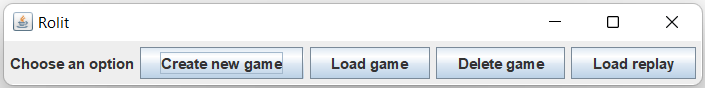
\includegraphics[scale=0.8]{menu-sprint3.png}
\end{center}

Inicialmente la ventana principal comienza con una pantalla en la que se muestran cuatro opciones a elegir por el usuario: \textit{Create new game, Load game, Delete game, Load replay}.

Si se ha decidido jugar a una partida o cargar una replay, el panel principal de la \textit{MainWindow} será reemplazado por un panel que contiene, de arriba a abajo, un ControlPanel, una TurnAndRankingBar, un BoardGUI y una StatusBar.

\begin{center}
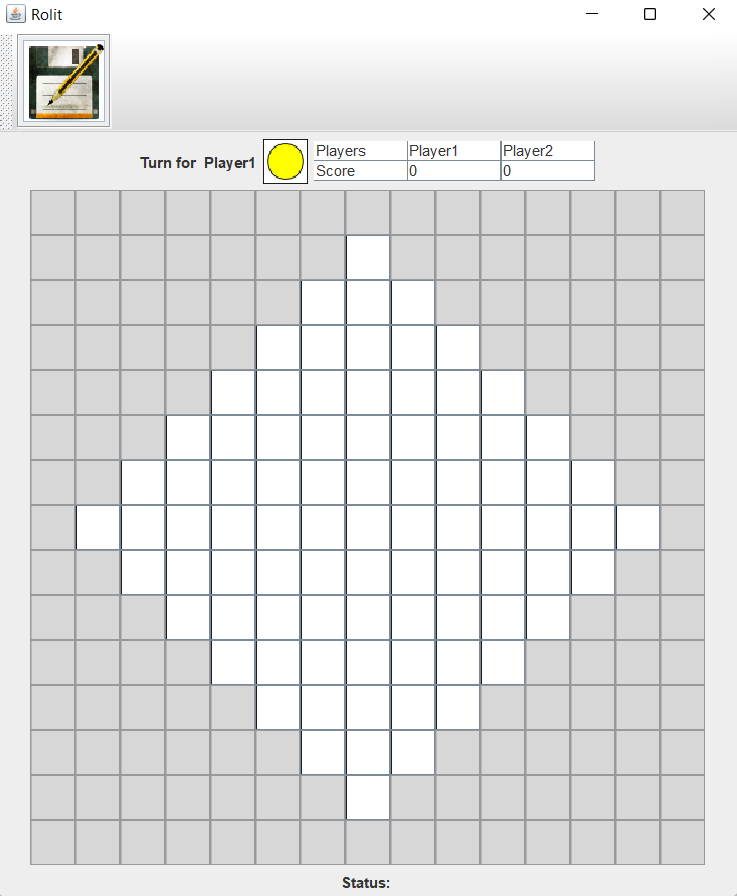
\includegraphics[scale=0.9]{game-sprint3.png}
%FIXME CENTRAR
Jugar una partida
\end{center}

\begin{center}
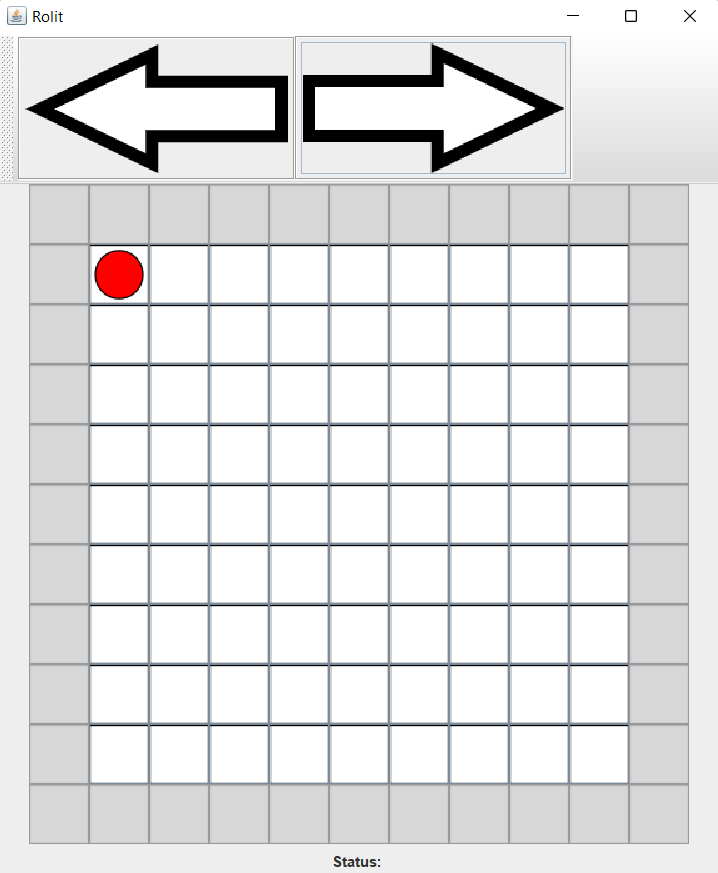
\includegraphics[scale=0.9]{replay-sprint3.png}
%FIXME CENTRAR
Reproducir una \textit{replay}
\end{center}

\underline{Funcionamiento interno}

Una vez visualizadas todas las pantallas es el momento de hablar su funcionamiento interno. Al introducir la GUI decidimos aplicar el patrón MVC, de manera que los futuros cambios en el modelo produzcan modificaciones mínimas en la vista y controlador y viceversa. Para más información sobre el Modelo-Vista-Controlador puede hacer click aquí. %FIXME AÑADIR REFERENCIA AL MVC

Para la comunicación de las vistas con los modelos se decidió utilizar el patrón observador, así son los propios modelos los que comunican a las vistas cuando deben actualizarse.

La implementación de este patrón se llevó a cabo mediante tres interfaces: Observable, diseñada para los modelos; RolitObserver, pensada para los observadores de la clase \textit{Game}; y ReplayObserver, que utilizan los observadores de la clase \textit{Replay}.

\begin{center}
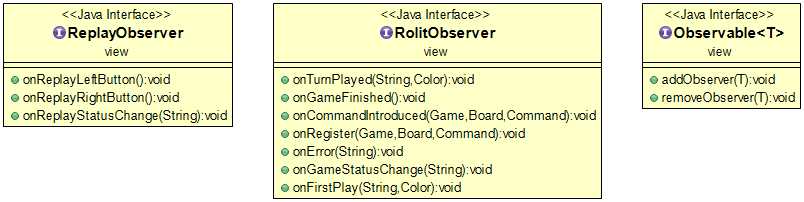
\includegraphics[scale=0.43]{observadores-sprint4.png}
\end{center}


En el caso de la GUI, la comunicación con los modelos se lleva a cabo a través de los \textit{ActionListeners} de los botones, que ejecutan el comando que corresponda.

\end{sprint}

\begin{sprint}[5]
\textbf{Console - JUANDI}

aaaaa

\textbf{GUI}

\underline{MainWindow}

La incorporación de la funcionalidad para jugar en red trajo consigo  la necesidad de añadir nuevos botones al menú principal para poder acceder a ella.

\begin{center}
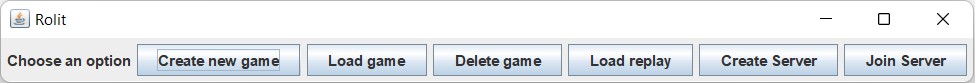
\includegraphics[scale=0.6]{menu-sprint5.png}
\end{center}

\underline{CreateGameDialog}

\begin{center}
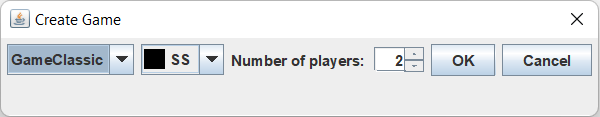
\includegraphics[scale=0.8]{create-game-sprint5.png}
\end{center}

Al configurar la partida de un servidor no es posible introducir la información de los jugadores, pues es cada uno individualmente quien decide su nombre y color desde su ordenador.

Por este motivo, se añadió un atributo al constructor de \textit{CreateGameDialog} que permite ocultar el panel que contiene los componentes para introducir los datos de los jugadores.

\underline{CreateServerDialog}
\begin{center}
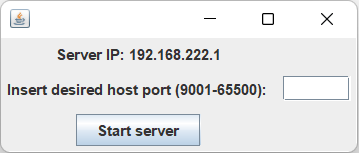
\includegraphics[scale=0.8]{create-server-sprint5.png}
\end{center}

Para poder crear el servidor el usuario debe elegir en qué puerto hostearlo, para ello se creó este \textit{JDialog}, que abre el servidor una vez se pulsa el botón ``Start Server".

En esta versión del juego, la poca experiencia con el manejo de hilos del equipo de desarrollo provocó que esta ventana se quedase pillada hasta que todos los participantes se unieran al servidor.

\underline{JoinServerDialog}
\begin{center}
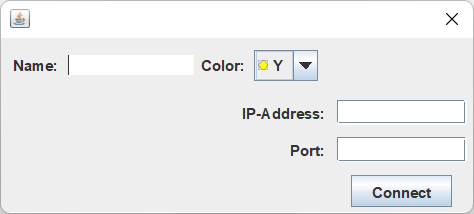
\includegraphics[scale=0.8]{join-server-sprint5.png}
\end{center}

Como ya se ha mencionado anteriormente, es cada usuario al unirse al servidor quien decide su nombre y su color. La clase \textit{JoinServerDialog} es la encargada de ello, además de recoger la IP y el puerto del servidor al que se quiere acceder.

\underline{Funcionamiento interno}

En el sprint anterior nuestra única intención era hacer una interfaz gráfica funcional, y ese objetivo fue alcanzado exitosamente. Sin embargo, la GUI accedía directamente a todos los métodos que necesitase de la clase \textit{Game}, algo que no es correcto desde el punto de vista de la programación orientada objetos.

Para solventar este problema planteamos inicialmente el uso de objetos transferencia que restringiesen los métodos de las clases que eran necesarias para visualizar el juego.

Finalmente, esta idea fue rechazada en favor de reutilizar el código ya existente. Así, se decidió que la información se transmitiese mediante la clase \textit{State} creada originalmente para reproducir las \textit{replays}, pues al fin y al cabo, un estado representa una serialización del juego y contiene toda la información necesaria.

\begin{center}
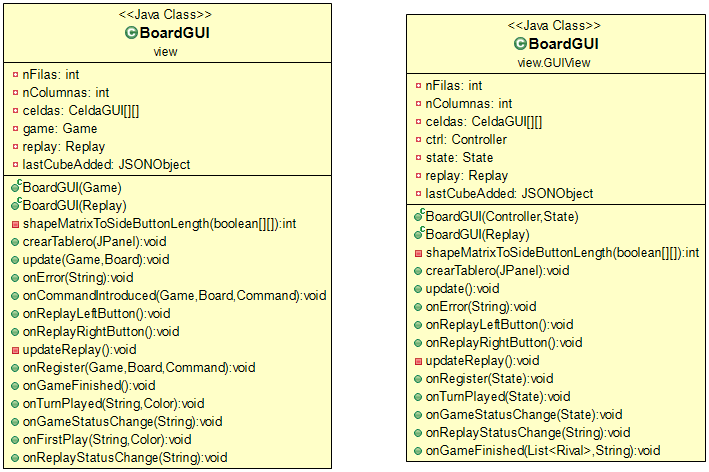
\includegraphics[scale=0.5]{board-gui-evol.png}

Evolución de la clase \textit{BoardGUI}. Sprint 4 (izq) y Sprint 5 (der)
\end{center}

Por consiguiente, todas las instancias de clases relacionadas con el modelo de \textit{Game} fueron eliminadas y reemplazadas por estados y JSONObjects. Para ello fue necesario añadir nuevos métodos a la clase \textit{State}.

\begin{center}
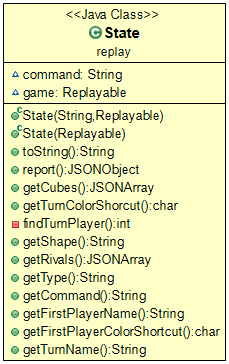
\includegraphics[scale=0.5]{state-sprint5.png}
\end{center}

\end{sprint}

\begin{sprint}[6]
\textbf{Console - JUANDI}

aaaaa

\textbf{GUI}

En este sprint la GUI fue refactorizada por completo, cambiando tanto visualmente, como a nivel de funcionamiento interno en algunas clases para hacer el código más manejable.

\underline{Creación de RolitComponents}

Hasta este momento el proyecto utilizada los componentes visuales de Java poder defecto, dando lugar a una interfaz gráfica funcional, pero con carencias visuales.

Para el estilo de los componentes, se optó por una interfaz minimalista basada en el color blanco y en el azul que aparece en el logo del juego Rolit, al que se denominó \textit{BLUE\_ROLIT}.

Los \textit{RolitComponents}, como la clase \textit{RolitButton} o \textit{RolitTextArea}, además de homogeneizar el entorno visual facilitan los cambios de estilo en un futuro.

Veamos el resultado gráfico tras la aplicación de estos componentes, sumado a re-estructuraciones en los Layouts y la inclusión de nuevas imágenes e iconos

\underline{MainWindow}
\begin{center}
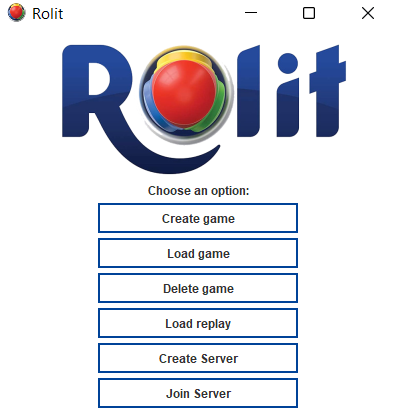
\includegraphics[scale=1]{menu-sprint-6.png}

\end{center}

\begin{center}
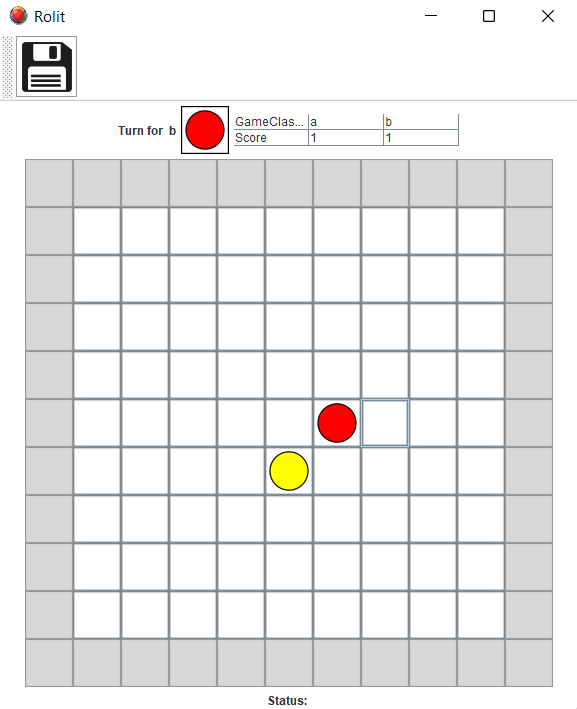
\includegraphics[scale=1]{partida-sprint-6.png}

Jugar una partida
\end{center}

\begin{center}
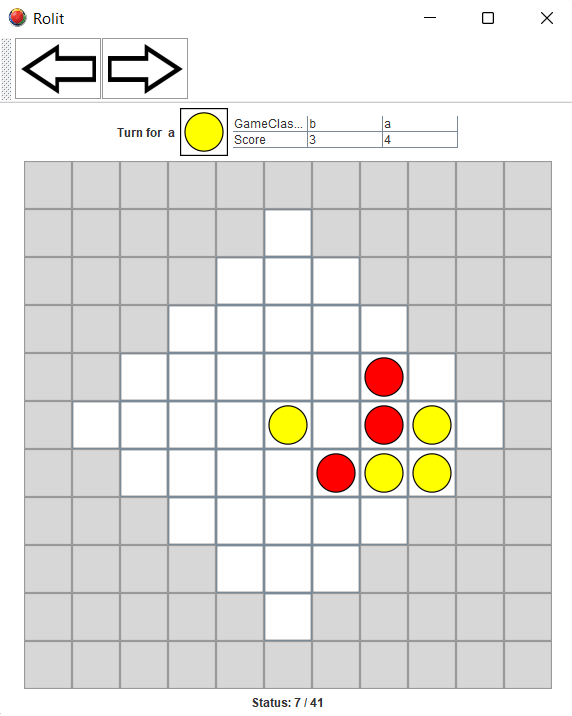
\includegraphics[scale=1]{replay-sprint-6.png}

Reproducir una \textit{replay}
\end{center}

\underline{CreateGame package}

En sprints anteriores había una clase encargada de crear y gestionar todos los componentes visuales necesarios para crear un juego nuevo, resultando en una clase demasiado compleja.

Por ello, la antigua clase \textit{CreateGameDialog}, fue dividida en otras más pequeñas. Dando lugar a:

\begin{itemize}
\item \textit{PlayerDataPanel}: panel que contiene los componentes necesarios para obtener la información de un jugador.
\begin{center}

\includegraphics[scale=1]{player-data-panel.png}
\end{center}
\item \textit{TeamDataPanel}: panel que contiene los componentes necesarios para obtener la información de un equipo.
\begin{center}

\includegraphics[scale=1]{team-data-panel.png}
\end{center}
\item \textit{CreatePlayersPanel}: conjunto de \textit{PlayerDataPanel}.
\item \textit{CreateTeamsPanel}: conjunto de \textit{TeamDataPanel}.
\item \textit{GameConfigurationPanel}: panel encargado de obtener la configuración básica del juego: modo de juego, forma, numero de jugadores...
\begin{center}
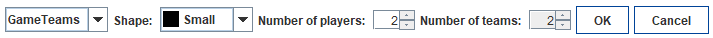
\includegraphics[scale=0.75]{game-config-panel.png}
\end{center}
\item \textit{CreateGameDialog}: ventana de diálogo que contiene un \textit{GameConfigurationPanel} y un \textit{CreateTeamsPanel}.
\begin{center}
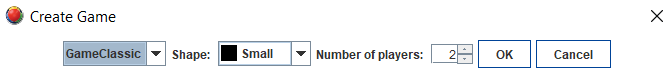
\includegraphics[scale=0.8]{create-game-sprint6.png}
\end{center}
\item \textit{CreateGameWithPlayersDialog}: extiende a \textit{CreateGameDialog}, añadiendo un \textit{CreatePlayersPanel}.
\begin{center}
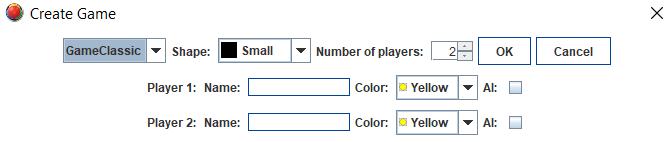
\includegraphics[scale=0.75]{create-game-players-sprint6.png}
\end{center}
\end{itemize}


\underline{LoadFileDialog}
\begin{center}
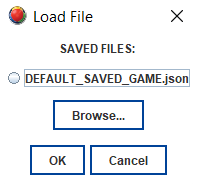
\includegraphics[scale=1]{load-game-sprint-6.png}
\end{center}

Las clases \textit{LoadGameDialog} y \textit{LoadReplayDialog} fueron abstraidas en \textit{LoadFileDialog}, que permite cargar tanto partidas como \textit{replays}, dependiendo del botón que se pulse.

\underline{DeleteGameDialog}
\begin{center}
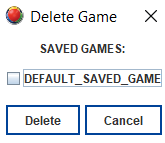
\includegraphics[scale=1]{delete-dialog-sprint6.png}
\end{center}

\underline{CreateServerDialog}

\begin{center}
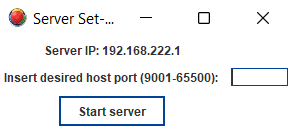
\includegraphics[scale=1]{server-setup-sprint-6.png}
\end{center}

Además, una vez creado el servidor, el usuario que está hosteandolo recibe feedback de cuanta gente se ha unido.

\begin{center}
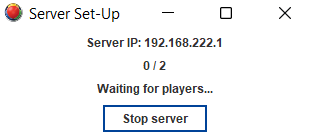
\includegraphics[scale=1]{server-feedback.png}
\end{center}


\end{sprint}

\underline{JoinServerDialog}
\begin{center}
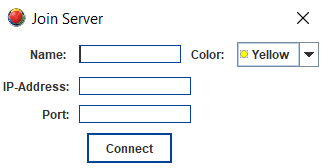
\includegraphics[scale=1]{join-server-sprint-6.png}
\end{center}

Los usuarios también reciben feedback del servidor, mostrándose una venta que les invita a esperar a los demás.

\begin{center}
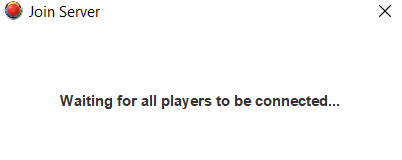
\includegraphics[scale=0.85]{user-feedback.png}
\end{center}

\subsection{Como usuario quiero que Rolit introduzca características innovadoras pensando en las posibilidades que brinda el multijugador}

\subsubsection{Como usuario, me gustaría que se pudiera jugar contra una inteligencia artificial, así como que ellas jugaran solas}
\begin{sprint}[5]
Este fue el Sprint en el que se empezaron a desarrollar las distintas estrategias de las inteligencias artificiales. Se planearon tres, recogidas en las siguiente clases, todas herederas de la clase abstracta Strategy: RandomStrategy, GreedyStrategy y MinimaxStrategy.

La idea de la estrategia es que, cuando le toque jugar a una inteligencia artificial, la estrategia se encarge de calcular
su siguiente movimiento y este se ejecutase inmediatamente después de su cálculo.

Para encapsular está lógica se creo la clase abstracta Strategy, para que cada estrategia en particular fuera una clase
heredera de esta.

Se han desarrollado tres estrategias, que suponen tres niveles de dificultad distintos, 
y la lógica de estas está recogida en las siguientes clases: RandomStrategy, GreedyStrategy y MinimaxStrategy.

\textbf{RandomStrategy}:
La idea es que se genere una posición cualquiera en el tablero, siempre y cuando esta sea válida. Esta es la posición que la inteligencia artificial jugará.
Lógicamente, la tendencia general las inteligencias artificiales que aplican esta estrategia es no obtener una gran cantidad de puntos, por lo que esta estrategia es la de nivel fácil.

\textbf{GreedyStrategy}:
Esta estrategia tiene por intención analizar el tablero en busca de la posición que le garantiza al jugador el máximo número de puntos en este mismo turno. Esta estrategia lleva a jugadas mucho mejores y elaboradas, pero sigue sin ser la mejor, así que representa el nivel de dificultad medio.

\textbf{MinimaxStrategy}:

Antes de explicar la implementación de esta estrategia en el caso de Rolit, debemos explicar primero en qué consiste la estrategia Minimax en teoría de juegos:

\textbf{Estrategia Minimax en teoría de juegos}: 

En teoría de juegos, el Minimax busca minimizar la pérdida esperada. La aproximación que se toma es asumir que el oponente va a tomar las decisiones que más te perjudiquen. De esta manera, al encontrar la decisión que menor pérdida suponga, el resultado real será siempre igual o mejor al calculado, de forma que el cálculo es fiable.

La mejor forma de explicar esto es a través de un ejemplo:

Imaginemos que estamos en un juego de dos jugadores, uno contra el otro, basado en turnos, en el cual ambos jugadores conocen en todo momento el estado actual de la partida en su totalidad. Un buen ejemplo de esto es el ajedrez. Supongamos pues que juegas con las piezas blancas, y tu adversario juega con las piezas negras. En cada uno de tus movimientos vas a jugar el movimiento que consideres que más te favorece. Por el otro lado, bajo nuestra aproximación, suponemos que el otro jugador va a jugar el movimiento que más te perjudique. Podemos hacer una representación de esto en forma de árbol:

Imaginemos que cada nodo contiene un número que representa el estado actual de la partida (para esto hace falta tener un criterio de valoración del estado actual de la partida, en el cual no entraremos en detalle en el caso del ajedrez, pero más adelante sí en el caso del Rolit), y cada arista representa un movimiento jugado, por el cuál se desciende en el árbol de un estado de la partida al siguiente. En cuanto a la valoración de los estados del juego, si el número de un nodo es positivo va ganando el jugador blanco (a mayor mejor); si el número es negativo, va ganando el jugador negro (a menor peor). Como el juego va por turnos, si un nivel del árbol se corresponde con el turno de un jugador, el siguiente nivel se corresponde con el siguiente jugador. De esta forma, volviendo al ejemplo propuesto, si desde un nodo se conoce el valor de todos sus descendientes pueden pasar dos cosas: si es el turno del jugador blanco, tomará la decisión que le lleve al mayor valor; si es el turno del jugador negro, tomará la decisión que le lleve al menor valor. 

Se ilustra el funcionamiento del algoritmo en la siguiente imagen: 

\begin{center}
\centering
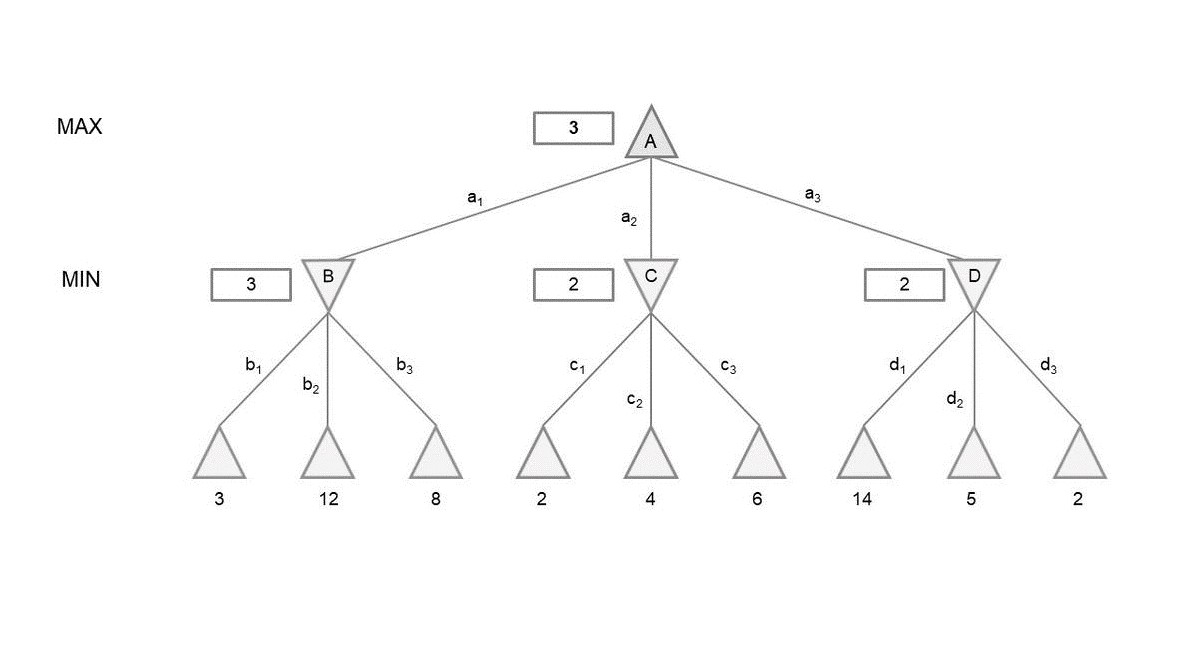
\includegraphics[scale=0.5]{minimaxExample.jpg}
\end{center}
%%FIXME Centrar

En el caso del ajedrez (y de la mayoría de juegos por turnos, como Rolit) hay siempre muchos posibles movimientos a jugar. De esta forma, en el árbol de decisión, de cada nodo salen muchos descendientes, resultando en un algoritmo con coste aproximadamente exponencial en el promedio de jugadas disponibles. Esto hace que la búsqueda del mejor posible movimiento se convierta en un problema intratable en no demasiados niveles de profundidad de búsqueda. Por tanto, surge la obligación de limitar la profundidad hasta la que se quiere hacer la búsqueda.

Volviendo ahora al Rolit, no estamos en un juego de dos jugadores (o al menos no necesariamente).
Afortunadamente, en este juego el criterio de valoración de jugadas es fácil: La mejor jugada es la que te lleve a acabar con el mayor número de puntos.

Ahora, como hay más de dos jugadores, para conseguir un cálculo de puntos fiable, el cálculo se lleva a cabo considerando que el jugador propietario de la estrategia quiere hacer aquella jugada que más puntos le otorgue a la larga, mientras que el resto de jugadores en sus turnos hacen la jugada que más puntos le quite al jugador propietario. De esta forma se calculan puntos para el jugador propietario situándonos en la situación más desfavorable posible, de forma que todo aquello que se calcule va a derivar siempre en un resultado igual o mejor al calculado, de forma que los resultados de los cálculos son fiables.

Debido a lo exhaustivos que resultan estos cálculos (y tras comprobación empírica simulando numerosas partidas) la estrategia MinimaxStrategy representa el nivel difícil de las inteligencias artificiales.

Ahora, antes de la explicación más técnica, observemos que la estrategia GreedyStrategy se puede implementar aplicando una MinimaxStrategy en la que solo se explora un nivel de profundidad, puesto que en este nivel se busca la jugada que más puntos garantice, y no se sigue buscando más allá. Por tanto, a nivel de clases, la clase GreedyStrategy es heredera de MinimaxStrategy, y el atributo de profundidad máxima pasa a valer 0.

Pasamos ahora a explicar la implementación de estas estrategias:

Para la simulación de movimientos pensamos originalmente en usar la clase Board para colocar cubos y evaluar resultados, pero no tardamos en darnos cuenta de que esto era inviable, puesto que los métodos de Board tienen una comunicación con otras clases que no deseeamos para esto, puesto que nosotros simplemente queremos hacer simulaciones, y no cambios reales.

Es por esto que fue necesario crear otra representación del tablero puramente funcional y adaptada a la simulación de movimientos, de donde surgió la siguiente clase:

\textbf{SimplifiedBoard}:

Esta clase consta de una matriz en la que almacena el color de los cubos del tablero real. Para disminuir costes y evitar tener que hacer copias del tablero tras cada movimiento simulado, se lleva una pila con los cambios que se realizan al simular un movimiento, de forma que cuando se quiere dejar el tablero en el estado previo a la simulación para realizar otra simulación, en vez de realizar una copia se revierten los cambios aplicados, lo cual resulta mucho menos costoso.

En SimplifiedBoard también se almacenan los puntos de los distintos jugadores, puesto que la idea es consultar los puntos después de simular cada movimiento.

Ahora, para calcular el mejor movimiento para ejecutar, en la clase de la estrategia se realiza un bucle en el que se recorren todas las posiciones del tablero, consultando si cada posición es válida o no, y en caso de dar con una posición válida, se simula ese movimiento.

Dentro de la simulación, en SimplfiedBoard, si la profunidad a explorar es mayor que 0, antes de revertir los cambios se vuelve a realizar el bucle de las posiciones, pero simulando esta vez para el siguiente jugador, y así hasta que la profundidad a explorar es 0. Hay que tener en cuenta que el jugador propietario de la estrategia busca maximizar sus puntos, mientras que el resto de jugadores buscan minimizarlos. Por tanto, en los bucles de recorrido de posiciones, la estrategia es conocedora de para qué jugador esta simulando el siguiente movimiento, de forma que si está simulando para el jugador propietario devolverá el resultado más favorable, y si está simulando para cualquier otro jugador devolverá el resultado más perjudicial posible para el propietario. De esta forma, se podrá conocer el resultado final realista de cada jugada posible, y así elegir la mejor jugada para el jugador propietario.

El cómputo del movimiento a jugar a través de la estrategia Minimax, llevado a cabo en el método calculateNextMove(), se ilustra en el siguiente diagrama:

\begin{center}
\centering
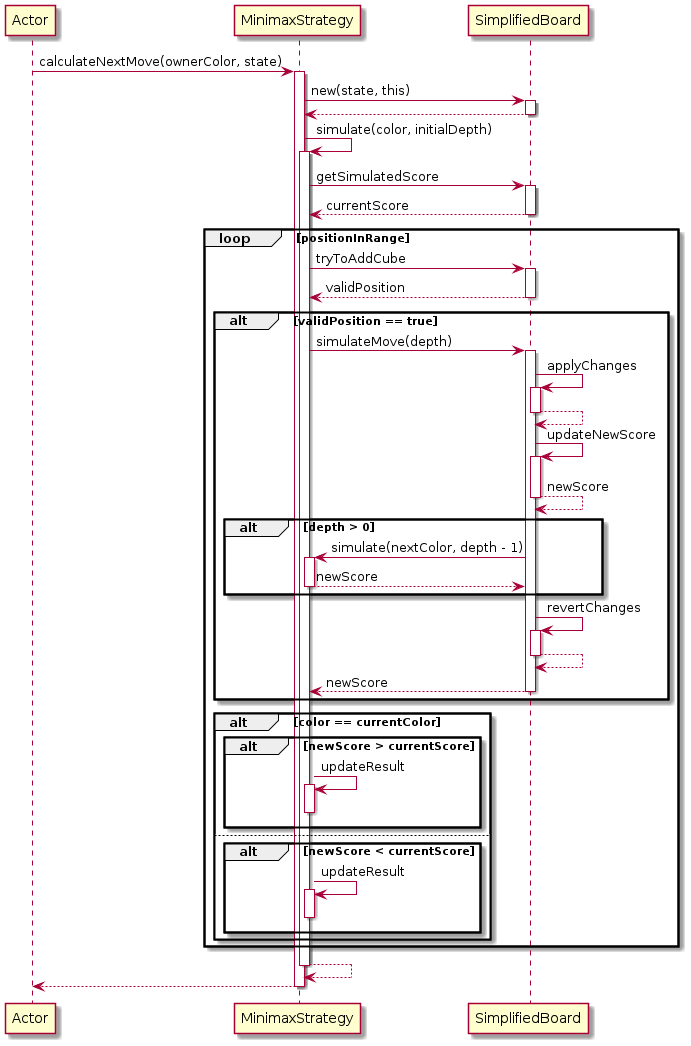
\includegraphics[scale=0.5]{Minimax.calculateNextMove()-Sprint5.png}
\end{center}

\end{sprint}

\begin{sprint}[6]
Por motivos de eficiencia de MinimaxStrategy, se ha implementado de forma complementaria la poda alfa-beta, que se explica a continuación:

\textbf{Poda alfa-beta}:
La poda alfa-beta es una mejora del algoritmo Minimax. Se mantienen dos valores, alfa y beta, que representan respectivamente la puntuación mínima que se llevará el jugador maximizador y la puntuación máxima que se asegura el jugador minimizados. Inicialmente, alfa es $-\infty$ y beta es $\infty$. 

Siempre que la puntuación máxima que se asegura al jugador que minimiza se vuelve menor que la puntuación mínima que se asegura el jugador que maximiza se puede parar de explorar por la rama actual. De forma análoga, se podan ramas en el caso contrario.

La mejor forma de visualizar esta poda es a través de una ilustración:

\begin{center}
\centering
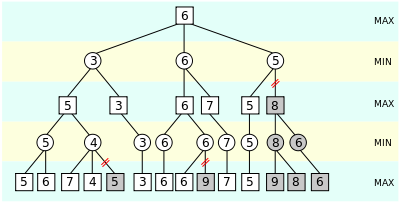
\includegraphics[scale=0.5]{poda alfa-beta.png}
\end{center}
%%FIXME Hacer más grande

Como vemos en este ejemplo, si exploramos en el árbol de izquierda a derecha, una verz llegamos a la rama derecha vemos que el jugador minimizador encuentra una rama por la que logra llegar al valor 5. Como minimiza, se sabe que el valor de ese nodo va a ser, como mucho, 5. Al ver esto el jugador maximizador, teniendo en cuenta que en una rama anterior ha llegado al valor 6, sabe que no tiene que seguir explorando esa rama, porque de ninguna manera va a encontrar un valor mejor que 6, y por tanto, en esta situación, el mejor resultado es el que le brinda empezar explorando la rama del centro.

Esta poda ha sido muy útil para reducir costes de cálculo, y el nuevo algoritmo mejorado queda reflejado en el siguiente diagrama:

\begin{center}
\centering
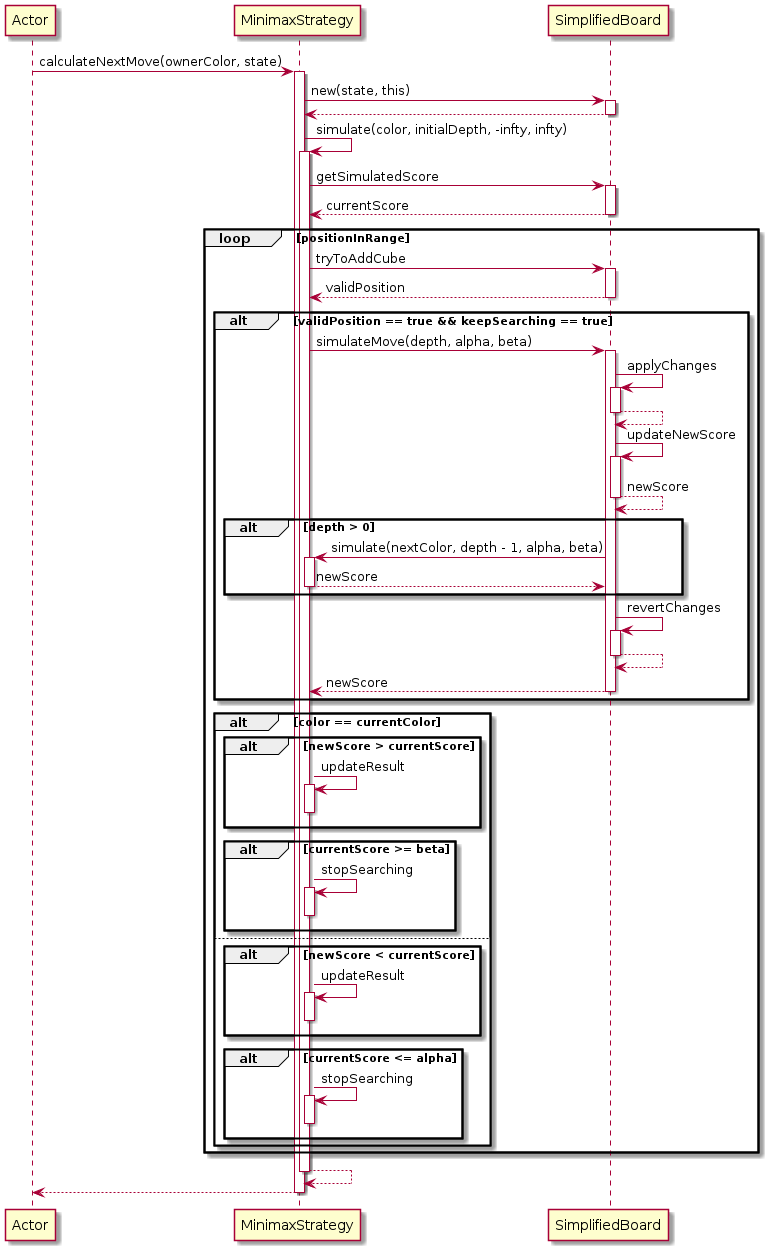
\includegraphics[scale=0.5]{Minimax.calculateNextMove()-Sprint6.png}
\end{center}

\end{sprint}

\subsubsection{Como usuario, me gustaría que se pudiera jugar en red.}
\begin{sprint}[5]
En cuanto a la tarea de añadir un modo de juego en red, se concibe, planea e implementa la funcionalidad de red casi por completo, consigue llegar a una versión funcional de juego en red en GameClassic. Al final del Sprint, los objetivos alcanzados son los siguientes:

\begin{itemize}
\item Determinar si el servidor, o por el contrario el cliente, debería poseer el modelo. Optamos por la segunda opción.

\item Definir toda la estructura en cuanto a relaciones jerárquicas de clases y dependencias entre las mismas.

\item Crear un número suficiente de diálogos en GUI que permitan la conexión en red. Entre ellos, se encuentran:
\begin{itemize}
\item ServerView
\item JoinServerDialog
\end{itemize}

El diseño y evolución pormenorizados de estos diálogos se encuentran en el apartado de la historia de usuario dedicada a la interfaz.

\item Reutilizamiento del código del diálogo de crear partida, adaptado a las circunstancias de red.

\item Poder jugar a una partida GameClassic en red de forma satisfactoria.

\end{itemize}

Aun así, otros de los objetivos propuestos no son implementados por falta de tiempo y de dependencia con otras de las partes del desarrollo no concluidos. Estos objetivos son:

\begin{itemize}
\item Crear más diálogos que aporten feedback para la conexión, tanto de la perspectiva del cliente como del servidor.

\item Llegar a una versión completamente refactorizada y con métodos simplificados.

\item Implementar el juego en red en GameTeams.
\end{itemize}

Fundamentalmente, la conexión en red se basa en una estructura en el que los clientes poseen el modelo, realizan cambios en el mismo y lo notifican al servidor. El servidor procede a enviar al resto de clientes la información nueva según la cual deben actualizar sus modelos. Nótese que el cliente sólo tiene contacto con el servidor, y el servidor tiene contacto con todos los clientes. Es, por tanto, un modelo de red centralizado, con nodo central el servidor.

\begin{center}
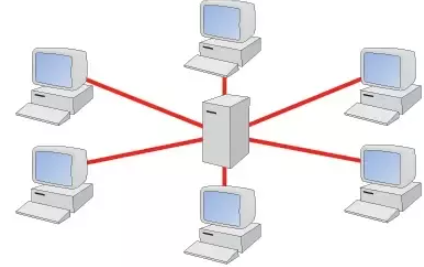
\includegraphics[scale=1]{redCentralizada.png} 
\end{center}

Para implementar esta funcionalidad de red en Java operamos según el modelo ServerSocket-Socket. Primero, desde la perspectiva del usuario que abre el servidor, se debe crear una instancia de ServerSocket pasándole como parámetro en el constructor el puerto en el que localmente debe operar el servidor. Posteriormente, se crea un nuevo Socket por medio de llamar al método accept() de ServerSocket. De esta forma, tenemos un socket asociado a un cliente en específico. Para n clientes el servidor necesitará n sockets. Cada cliente solo necesita un socket, pues solo tiene conexión con el servidor y no con el resto de clientes.

\begin{lstlisting}[frame=single, language=Java]
//Perspectiva del servidor

ServerSocket serverSocket = new ServerSocket(port);
Socket socketCliente1 = serverSocket.accept();
...
...
...
Socket socketClienteN = serverSocket.accept();

\end{lstlisting}


Este método accept() se queda "bloqueado" o en espera, hasta que un cliente se conecta por medio de la creación de un Socket desde su aplicación de la siguiente manera:

\begin{lstlisting}[frame=single, language=Java]
//Perspectiva del cliente

Socket socket = new Socket(ip, port);

\end{lstlisting}

donde ip es la dirección IP donde opera el servidor (ya sea local, o pública con el puerto especificado abierto para permitir conexiones desde fuera de su red), y port el puerto donde esta opera.

Una vez que las creaciones del Socket de servidor y cliente han sido creadas de forma satisfactoria, la conexión ha sido realizada con éxito. Por tanto, podemos proceder al envío de mensajes entre cliente-servidor y viceversa.

Para ello, Java nos ofrece realizar este cambio de información por medio de pares de instancias BufferedReader-PrintWriter, llamémosle in e out respectivamente. Estas instancias leen y reciben String, respectivamente. Nuestro modelo procederá a enviar JSONObject pasados a formatos String, que después al ser recibidos como Strings se volverán a construir en JSONObject por medio de la constructora de JSONObject que admite como parámetro un String.

Cada servidor posee un número de parejas in-out equivalente al número de clientes conectados, y cada cliente posee una pareja.

\begin{lstlisting}[frame=single, language=Java]
//Perspectiva del servidor
BufferedReader inCliente1 =  new BufferedReader(new
InputStreamReader(socketCliente1.getInputStream()));
...
...
...
PrintWriter outClienteN =  new PrintWriter(
socketClienteN.getOutputStream(), true);
\end{lstlisting}

\begin{lstlisting}[frame=single, language=Java]
//Perspectiva del cliente
BufferedReader in =  new BufferedReader(new
InputStreamReader(socket.getInputStream()));

PrintWriter out =  new PrintWriter(
socket.getOutputStream(), true);
\end{lstlisting}


De esta forma, cada vez que se pretende enviar un mensaje desde el cliente al servidor, el cliente k envía un mensaje msg por medio del método out.println(msg). Este mensaje es recogido desde el servidor por el método inClienteK.readline(). Asimismo, si el servidor pretende enviar un mensaje al cliente k, este debe llamar a outK.println(msg). El cliente k recoge el mensaje desde in.readline(). En resumen:

\begin{lstlisting}[frame=single, language=Java]

	//Envio de mensaje ClienteK Servidor


//Perspectiva del cliente k
out.println(msg);

--->

//Perspectiva del servidor
String msg = inClienteK.readline();



	//Envio de mensaje Servidor-ClienteK


//Perspectiva del servidor
outK.println(msg);

-->

//Perspectiva del cliente k
String msg = in.readline();
\end{lstlisting}

Sin embargo, surgen una serie de problemas con respecto a este modelo. El servidor debería recibir de manera independiente, paralela y en cualquier momento los peticiones de cada cliente, de lo contrario habría que definir un orden completamente arbitrario de llegada de mensajes según cliente. Si bien esto pudiera hacerse para realizar juegos por turnos en el que un mensaje enviado por un cliente al que no le corresponde el turno no sea procesado por el servidor, otras funcionalidades serían imposibles de implementar.

Por ejemplo, podría ocurrir que en el modo por equipos, dos clientes se conecten. Reciben ambos del servidor una lista de equipos en la que pueden conectarse. Se ve que es absurdo imponer un orden de quién envía la información del equipo elegido, pues esta es imposible de anticipar. Puede darse que el primer cliente que se conecte sea el segundo que especifique en qué equipo quiere conectarse.

En suma, nos interesa que la llegada de mensajes no deba ser regida por un orden definido y arbitrario. Para ello, nos interesa utilizar una herramienta de la programación concurrente y paralela, los hilos; en el caso de Java, proporcionados por la clase Thread.

De esta manera, si el servidor tiene un hilo por cada cliente, podrá recibir mensajes de forma paralela. Así, ningún mensaje enviado desde un cliente es perdido; todos llegan al servidor con independencia de cuándo se emitan desde el cliente. Desde la perspectiva del servidor, este es el cometido de la clase ServerClientThread implementada en el proyecto, que extiende de Thread. En su método run, recibe mensajes con el método readLine() anteriormente descrito \textbf{de forma periódica y constantemente (en un while), hasta que se haya decidido cerrar el juego}. Posteriormente, se envía este mensaje al método receiveFromClient, synchronized (pretendemos ejecutar múltiples procesamientos que de forma secuencial para evitar errores imprevistos), que pertenece a la clase Server, que de forma sincronizada procesa este mensaje.

El cliente se encuentra en una situación parecida. ¿Qué ocurre si recibe una información del servidor, la procesa y mientras se da este procesamiento, recibe otro mensaje del servidor? Necesitará el cliente, por tanto, dos hilos: un hilo que se dedique a recoger mensajes, y otro hilo que se dedique a procesarlos. De esta forma, ninguna información emitida desde el servidor es perdida.

Una vez el modelo de red ha sido completamente explicado, procedemos a detallar los detalles de implementación relativos al juego en específico. Es preciso introducir el diagrama de clases relativo a este Sprint.

\begin{center}
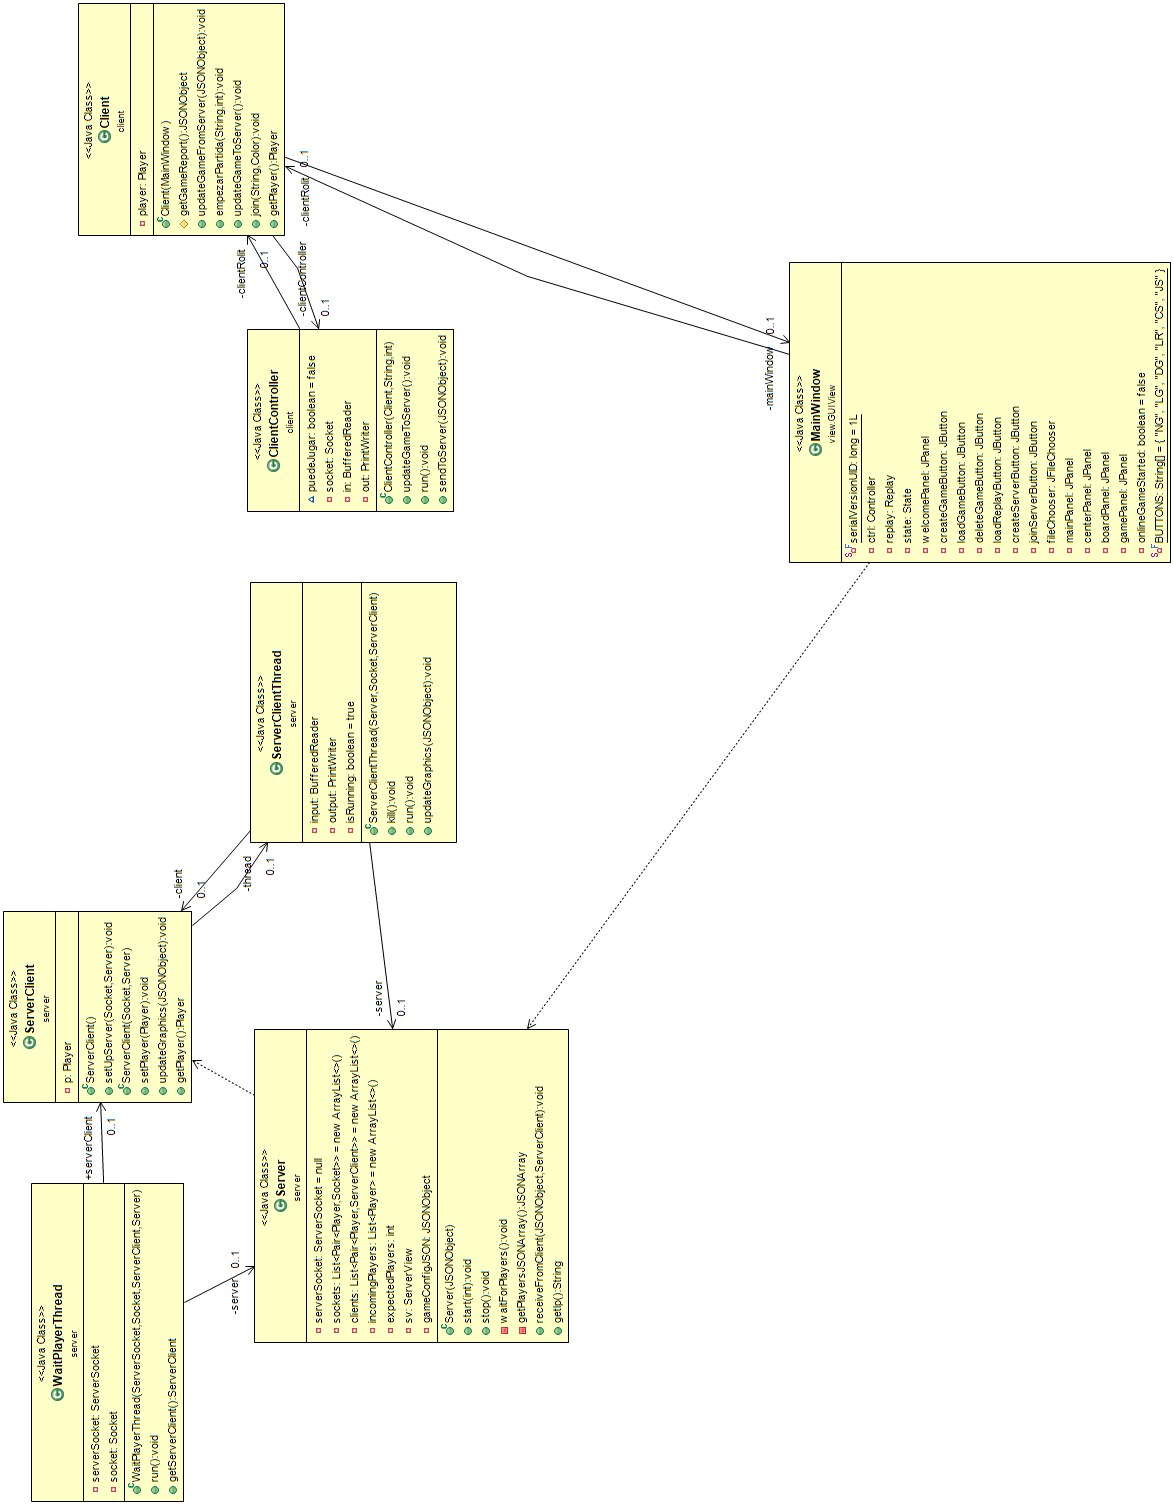
\includegraphics[scale=0.25]{UMLClasesRedSprint5.png} 
\end{center}

Empezamos a detallar la estructura del servidor.

ServerView, especificado en el apartado de diseño correspondiente, tiene el papel de pasar la información pertinente para el funcionamiento de la clase Server.

Partimos de la clase Server, clase que gestiona los clientes desde la perspectiva del servidor y que procesa los mensajes emitidos desde los clientes.

\begin{center}
\includegraphics[scale=0.3]{Server-sprint5.png} 
\end{center}

Como hemos anticipado, Server debe poseer un único ServerSocket a través del cual se abre el servidor. Posee el atributo expectedPlayers recibido desde la GUI, en el que el usuario que ha abierto el servidor especifica qué número de jugadores se conectarán al servidor. Es de vital importancia conocer este dato, pues de ello dependerá el número de WaitPlayerThread creados, clase que pasaremos a comentar después.

Asimismo, Server posee dos listas: una correspondiente a pares Player-Socket, de modo que a cada jugador se le asocia el Socket a través del cuál puede comunicarse con el cliente en específico que juega bajo su identidad; y otra correspondiente a pares Player-ServerClient, donde a cada jugador se le asocia el ServerClient específico. Pasaremos a describir posteriormente qué es la clase ServerClient.
En resumen, tenemos asociaciones biunívocas jugador-cliente las cuales aprovecharemos para el envío y la recepción de mensajes.


El ServerClient constituye una representación de un cliente en específico desde la perspectiva del servidor. 

\begin{center}
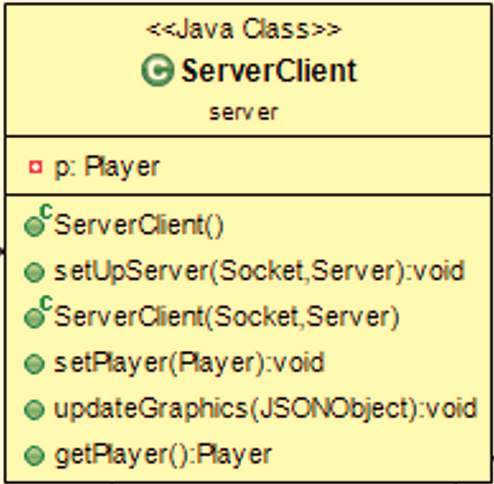
\includegraphics[scale=0.3]{ServerClient-sprint5.png} 
\end{center}

Lo fundamental de la clase ServerClient es que posee el thread encargado de la recepción directa de mensajes desde el cliente en específico; es decir, posee una única instancia de clase ServerClientThread, anteriormente mencionada.

\begin{center}
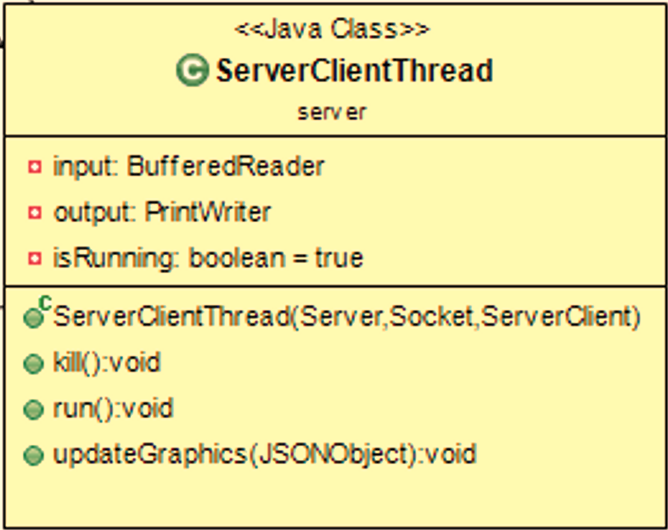
\includegraphics[scale=0.3]{ServerClientThread-sprint5.png} 
\end{center}

ServerClient posee una referencia a su ServerClientThread y viceversa. Esto es porque:

\begin{itemize}
\item ServerClient posee a ServerClientThread porque el servidor, al enviar mensajes al cliente, pasa el mensaje por ServerClient (recordemos la lista Player-ServerClient) quien pasa a enviárselo a a ServerClientThread.
\item ServerClientThread posee a ServerClient porque al recibir mensajes desde el cliente, ServerClientThread envía el mensaje a Server para procesarlo. En esta función server.receiveFromClient, se necesitan dos parámetros: el mensaje, y el ServerClient asociado. Es por esto que para este segundo parámetro, ServerClientThread necesite una referencia de ServerClient.
\end{itemize}

Como vemos, la finalidad es encapsular el código de forma que Server no conozca de ServerClientThread sino solo de ServerClient.

WaitPlayerThread, por otra parte, es un hilo encargado de ir recibiendo los jugadores.

\begin{center}
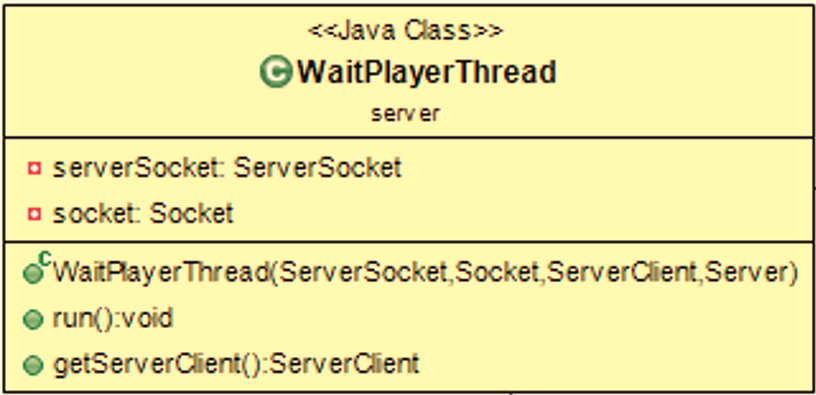
\includegraphics[scale=0.3]{WaitPlayerThread-sprint5.png} 
\end{center}

Se crean un número "expectedPlayers" (atributo de Server) de instancias de esta clase, cada una de ellas con un ServerClient asociado (por tanto, ServerClient es atributo de WaitPlayerThread). En su método run se encarga de ejecutar el método serverSocket.accept() que especificamos anteriormente. En cuanto se acepta la conexión, se procede a llamar al método setUpServer de ServerClient para que este cree su ServerClientThread.

La necesidad de hacer esto de forma paralela justifica la creación del hilo WaitPlayerThread. Para evitar problemas de concurrencia, en esta clase los atributos Server y ServerClient son volátiles para que todos los hilos WaitPlayerThread conozcan en tiempo real el estado de Server y ServerClient.

En particular, Server debe ser volatile pues debe ir actualizando su lista de Player-Socket en tiempo real y de forma organizada de a fin de evitar bugs. Esto es porque el método sincronizado waitForPlayers de Server recoge periódicamente el número de conexiones aceptadas. En cuanto estas conexiones igualan el número de conexiones aceptadas, el método deja de ejecutarse y se procede a las gestiones que tiene que realizar el servidor una vez todos los usuarios esperados se han conectado.

Una vez detallados los cometidos de todas las clases que posee el servidor, pasamos a detallar las del cliente.

El punto de partida es la clase Client, que será un intermediario entre su thread de recepción de mensajes y la GUI.

\begin{center}
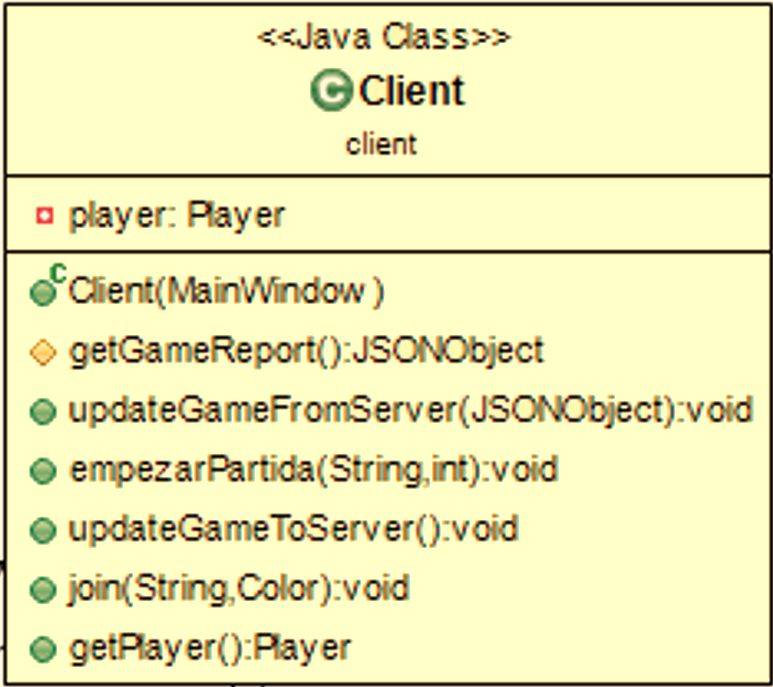
\includegraphics[scale=0.3]{Client-sprint5.png} 
\end{center}

Como Client es un intermediario, MainWindow precisa una referencia de Client y Client una de MainWindow; es decir, la comunicación es bidireccional. La razón de esto es:

\begin{itemize}
\item Al hacerse una jugada en el modelo, como se ha especificado, necesitamos pasar el nuevo estado del juego al servidor para que este, a su vez, se la pase al resto de clientes. Por tanto, MainWindow pasa el estado del juego a su Client. MainWindow, a su vez, obtiene este estado del juego desde el controlador. Todos estos pasos de información se realizan a través de los métodos updateGameToServer que poseen estas clases.

\item Al recibirse un nuevo estado del juego desde el servidor, Client recibe esta información desde su thread. Necesita a MainWindow para que este, a su vez, envíe el nuevo estado del juego al controlador con el fin de actualizar el modelo al nuevo juego requerido. Todos estos pasos de información se realizan a través de los métodos updateGameFromServer que poseen estas clases.
\end{itemize}

Finalmente, pasamos a describir ClientController, el thread de Client.

\begin{center}
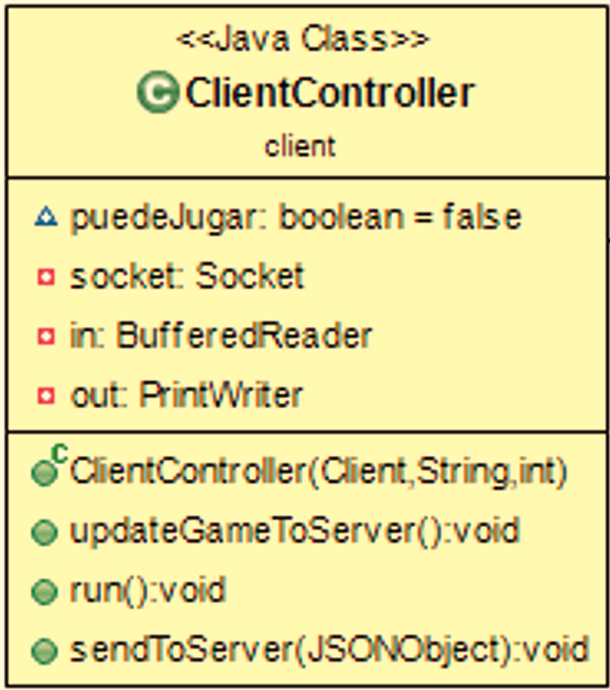
\includegraphics[scale=0.3]{ClientController-sprint5.png} 
\end{center}

Nuevamente la comunicación entre Client y ClientController es bidireccional: para enviar información al servidor, Client notifica a ClientController; para recibir información del servidor, ClientController notifica a Client.

Como hemos anticipado, ClientController extiende de Thread, y en su método run() recibe información del servidor que procede a enviar al cliente. El método sendToServer envía la información directamente al servidor por medio de out.println como hemos descrito.

Una vez especificadas todas las clases, describiremos el hilo típico de la ejecución para comprender cómo operan estas y en el orden en el que lo hacen.

\begin{center}
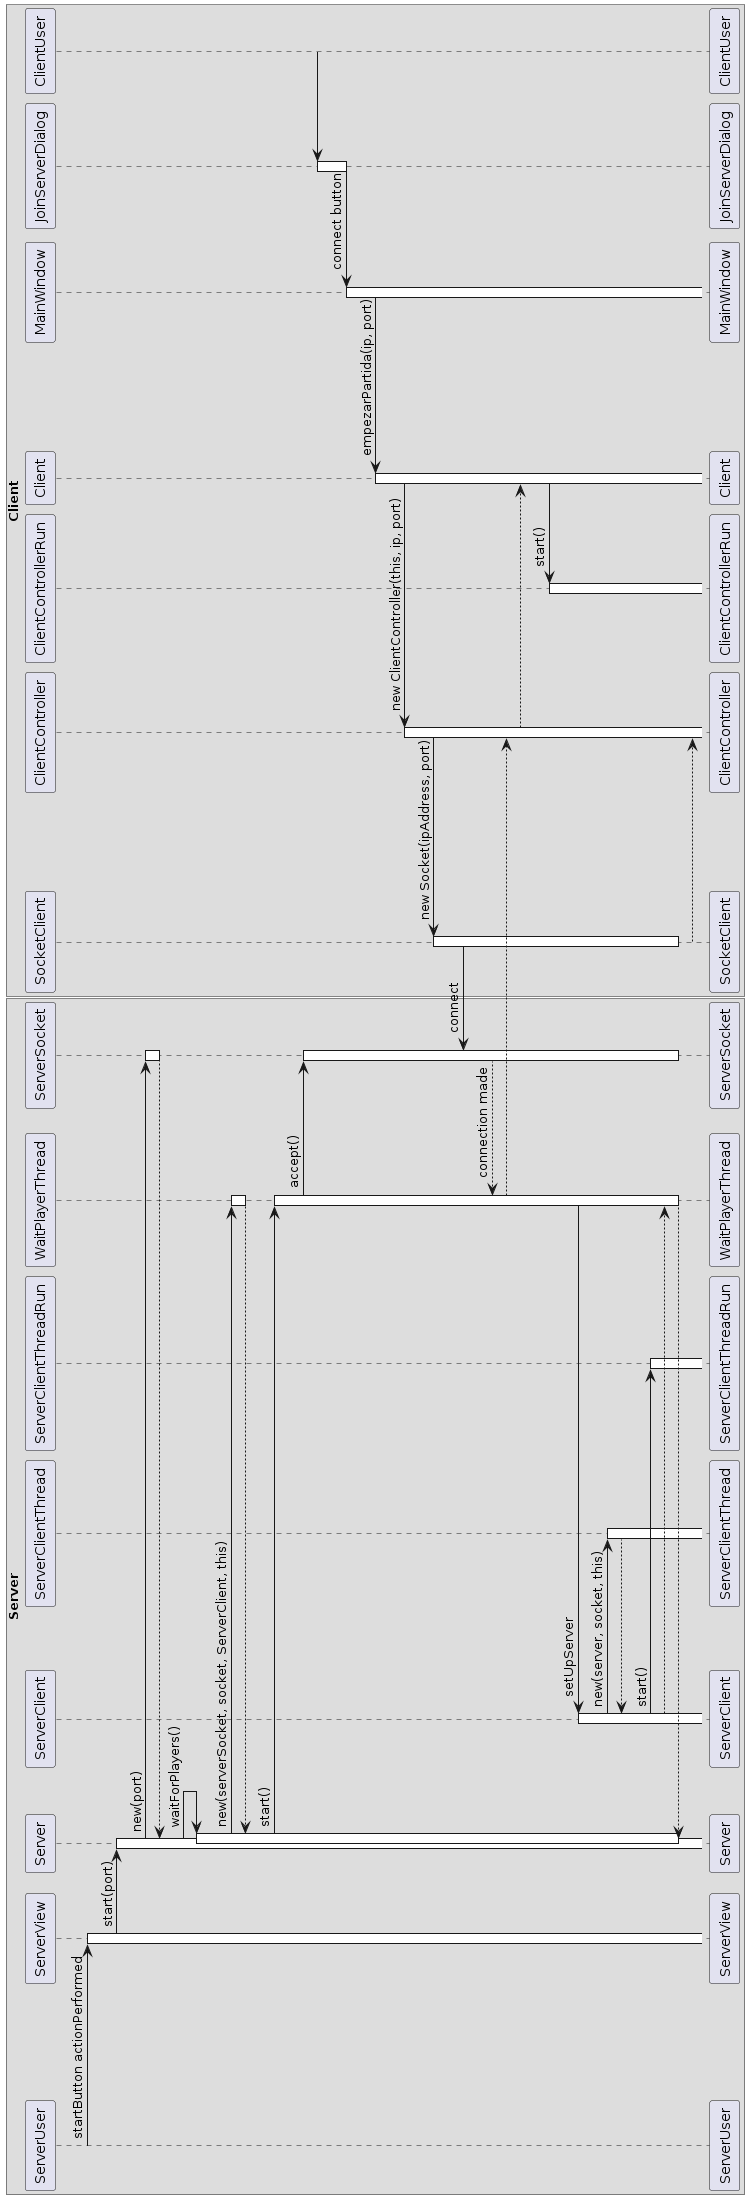
\includegraphics[scale=0.2]{umlconexiones.png}
\end{center}

Observamos que al pulsar el botón de Start Server en el diálogo de abrir un servidor, se llama crea Server pasándole como parámetro un JSON (gameConfigJSON) correspondiente a una configuración del juego básica especificada desde la GUI, que el servidor rellenará añadiendo los jugadores pertinentes.
En el constructor de Server se almacena este atributo JSON y se llama al método start(port) que crea el ServerSocket. Posteriormente, llamada al método waitForPlayers para realizar las conexiones oportunas.
Este método se compone de un bucle for que recorre un número de vueltas equivalente al del número de jugadores a conectarse esperados. por cada vuelta, se crea su ServerClient y Client asociados, y se crea el thread WaitPlayerThread y se llama a start(). El WaitPlayerThread, en su método run() llamado desde start(), espera en el método de serverSocket.accept() que se conecte un cliente.

Un cliente, por medio de JoinServerDialog, se conecta al servidor desde la IP y puerto requeridos. Pasa por el MainWindow quien a su vez llega al cliente (Client) con el método empezarPartida, en base a las relaciones ya descritas. El cliente crea su thread ClientController. En la constructora de ClientController se realiza la conexión al servidor mediante la creación del Socket.

En cuanto esta se realiza con éxito, ocurren dos procesos de forma paralela:

\begin{itemize}
\item En el servidor, el método serverSocket.accept() es ejecutado con éxito. Se procede a llamar al método setUpServer del ServerClient específico asociado a esta conexión; se crea después un thread ServerClientThread el cual crea los BufferedReader y PrintWriter oportunos, y ServerClient procede a llamar al run() de este thread (representado en la lifeline ServerClientThreadRun)

\item En el cliente, una vez se ha creado el Socket con éxito en la constructora de ClientController, se crean los BufferedReader y PrintWriter oportunos. Se termina la constructora, y acto seguido Client llama al start de ClientController para que empiece a recibir mensajes en su método run().
\end{itemize}

Si la conexión no se ha realizado bien, se generan las excepciones oportunas que cierran las ventanas de tanto cliente como servidor.

El thread WaitPlayerThread procede a esperar un segundo antes de cerrarse. En este segundo, se espera que el cliente envíe al servidor la información relativa al Player (qué color y qué nombre ha escogido). Esta información pasa a registrarse en la lista de incomingPlayers de forma síncrona mientras WaitPlayerThread espera. El mecanismo pormenorizado es el siguiente:

\begin{center}
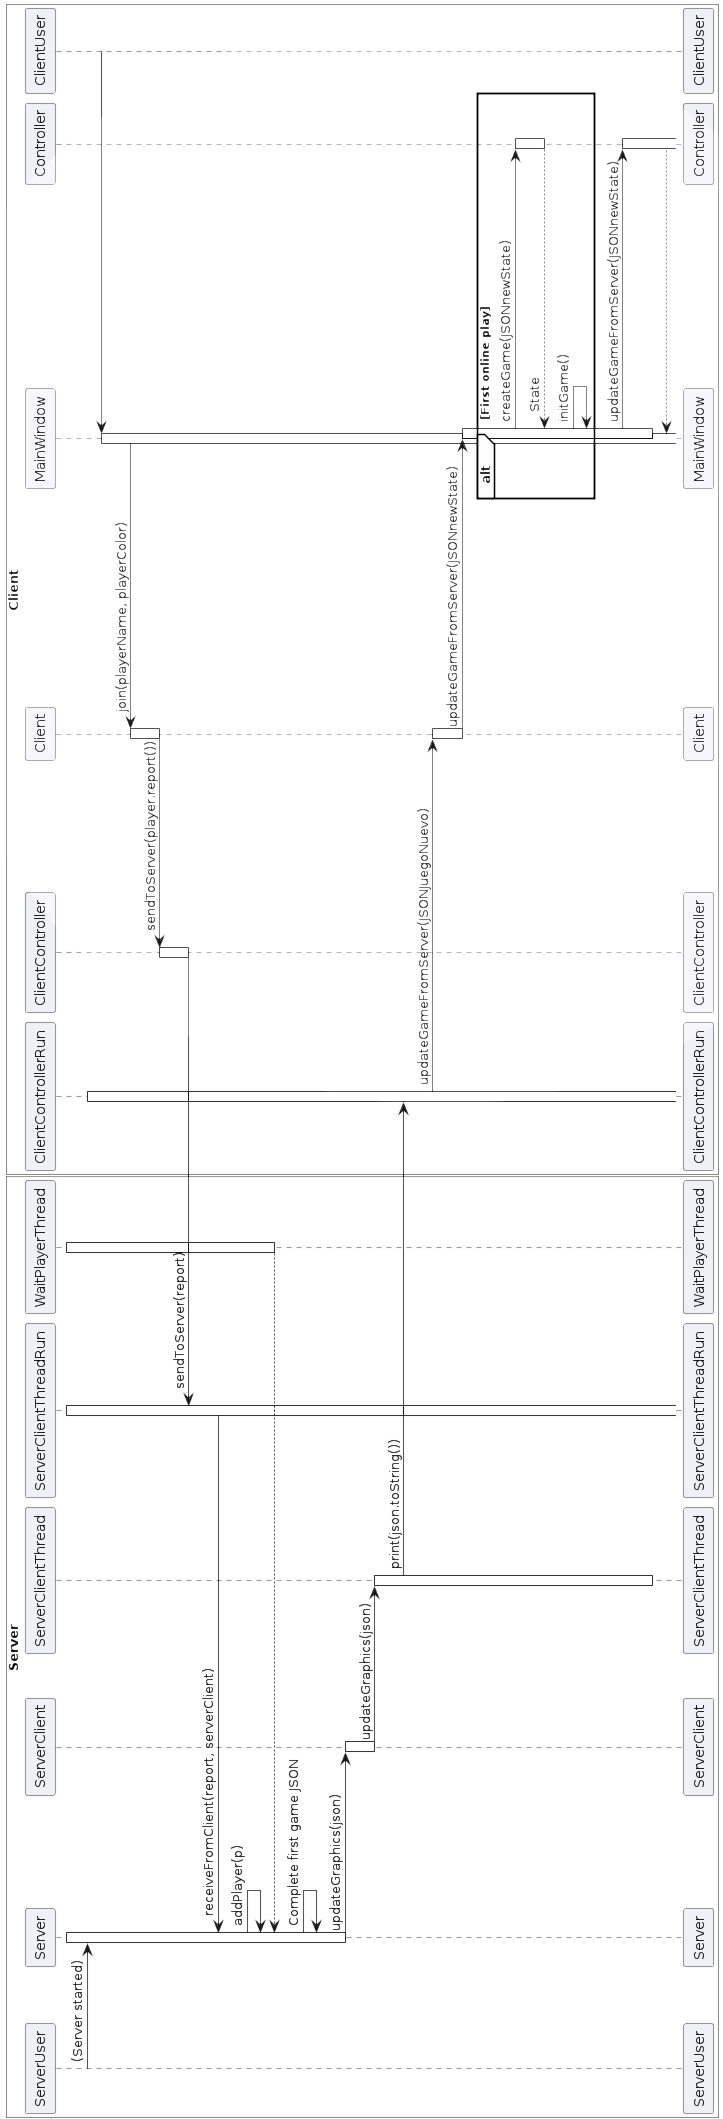
\includegraphics[scale=0.2]{empezarPartidaUml.png}
\end{center}

\begin{enumerate}
\item Tras ejecutarse el hilo ClientController, el método empezarPartida de Client se finaliza. MainWindow procede a ejecutar el método join de Client, pasándole como argumentos el nombre y color escogidos.
\item Client pide al thread ClientController que envíe al servidor esta información.
\item ClientController envía la información por medio del método sendToServer
\item El ServerClientThread específico asociado al cliente que envía esta información recibe en su método run el mensaje. Procede a llamar al método asíncrono receiveFromClient de Server.
\item receiveFromClient distingue, observando el JSONObject enviado, si se trata de información de actualización de juego o información respecto a un nuevo jugador añadido. En el caso que nos ocupa, es esta segunda opción; receiveFromClient procede a crear una instancia de Player y añadirla a incomingPlayers (ArrayList de Player).
\end{enumerate}

Todo este proceso tarda (bastante) menos del segundo que espera WaitPlayerThread; se deja un segundo de cortesía para dar un amplio margen a los equipos más lentos.

El método run() de WaitPlayerThread se finaliza y se ejecuta desde waitForPlayers (Server) el método join para que concluya el thread.

Dado la información obtenida de Socket, ServerClient y Player (este último con incomingPlayers, cuyo último elemento añadido es el Player correspondiente al cliente), se rellenan las dos listas Player-Socket y ServerClient-Player de Server con una nueva posición.

Todo esto es una única vuelta del bucle de waitForPlayers. Como hemos comentado, se ejecutarían un número de vueltas equivalente al número de jugadores esperados.

Una vez todos los jugadores se han conectados y las dos listas completadas, se sale del bucle y waitForPlayers procede a crear rellenar el incompleto gameConfigJSON que fue pasado con anterioridad por el constructor de Server; ahora es el momento correcto para hacerlo pues ya se conoce la información de todos los players. Se rellenan los campos pertinentes previamente incompletos de gameConfigJSON; posteriormente, se envía este primer estado del juego a todos los clientes por medio del método updateGraphics.

El cliente recibe esta configuración del juego en su thread, se llama al método updateGameFromServer de Client, quien a su vez llama a updateGameFromServer de MainWindow.

En este último método, si es la primera jugada, se llama crea el juego en el controlador, y después se llama a initGame() para inicializar las componentes visuales relativas al juego.
En cualquier caso, se llama después al método updateGameFromServer de Controller para actualizar el juego tal y como ordena el JSON pasado como parámetro.

Los mecanismos de este método son crear un nuevo juego a partir del nuevo JSON estado del juego, pasar los observadores del Game antiguo al nuevo, y adjudicar al atributo Game de Controller este nuevo juego.

\begin{lstlisting}[frame=single, language=Java]
public void updateGameFromServer(JSONObject o) {
  Game newGame = GameBuilder.createGame(o);
  newGame.updateGameFromServer(game.getObserverList());
  game = newGame;
}
\end{lstlisting}

Falta por especificar cómo se produce una jugada en el modo online y cómo evitar que los clientes jueguen cuando no es su turno.

\begin{center}
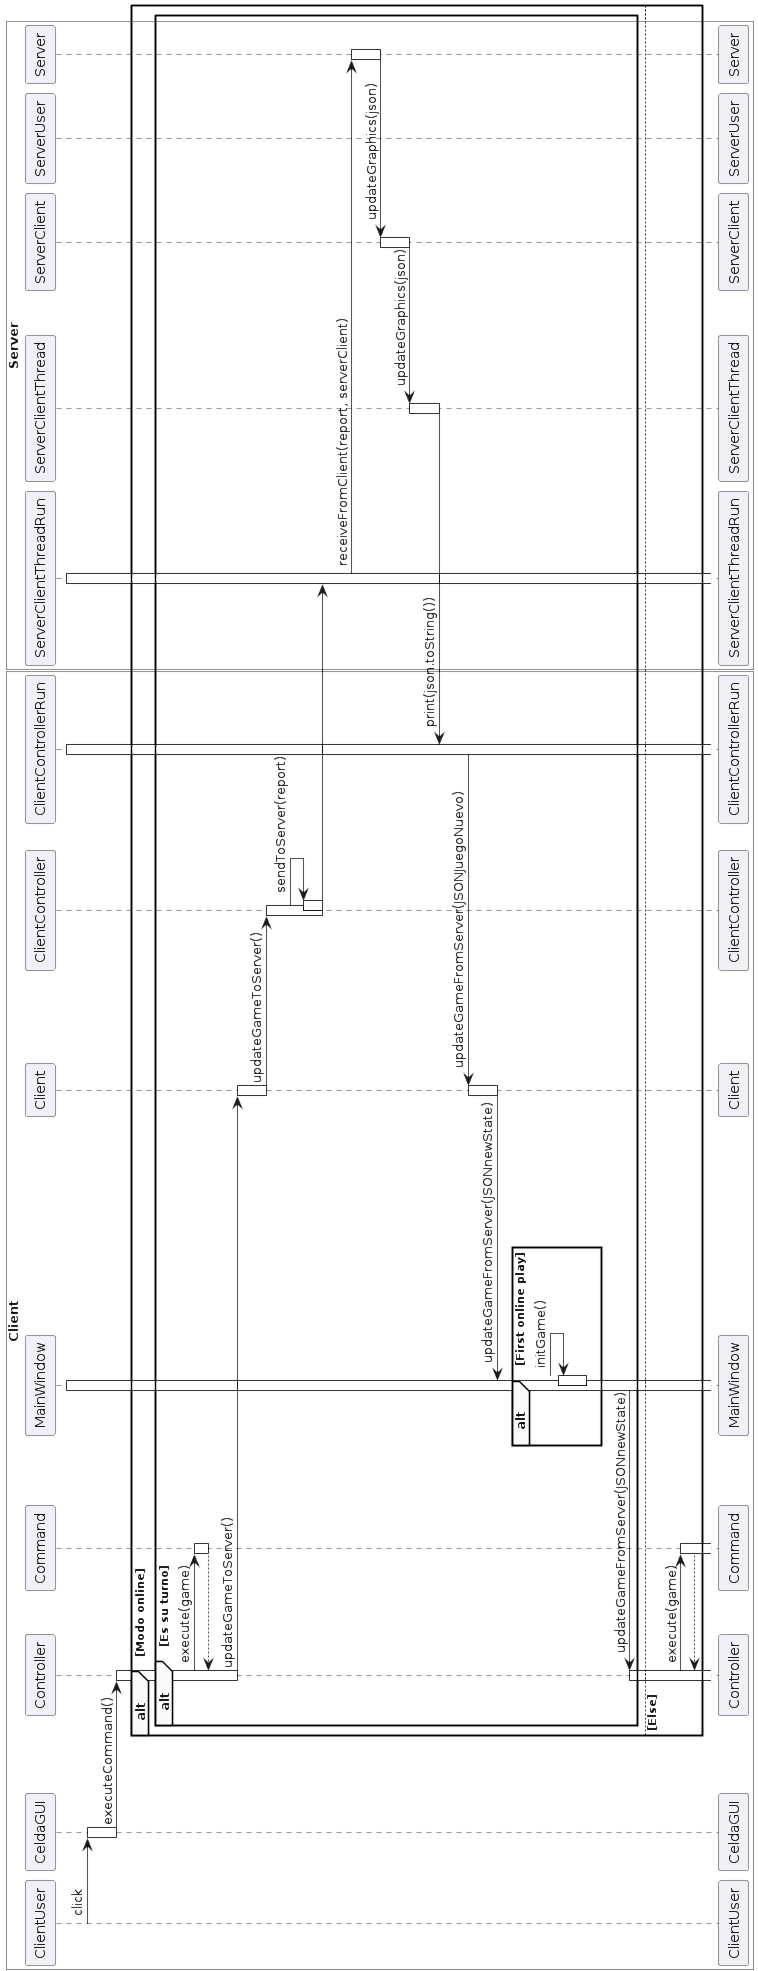
\includegraphics[scale=0.2]{juegoTipicoUml.png}
\end{center}

Se pulsa una celda en el tablero y se pide al controlador que ejecute el comando de poner cubo en la posición pedida, como de costumbre. En caso de que se juegue el modo online, se comprueba si el jugador está legitimado para jugar (es decir, es su turno). Para ello, se comprueba que el jugador turno del juego es el mismo que el jugador del cliente (recordemos que Client tiene el atributo Player del jugador al que corresponde).

De verificarse estas dos condiciones, se ejecuta el comando y se envía el nuevo estado del juego al servidor, quien enviará este nuevo estado al resto de clientes.

De no jugarse el modo online, se ejecuta el comando como de costumbre.

\begin{lstlisting}[frame=single, language=Java]
if (onlineMode) {
			
 if (game.getCurrentPlayer().getColor()
 .equals(clientRolit.getPlayer().getColor())) {
   command.execute(game);
   clientRolit.updateGameToServer();
 }
			
}
else
 command.execute(game);
\end{lstlisting}

Nótese que este último diagrama de secuencia se representa a Client como entidad abstracta emisora y receptora, realmente un Client sería emisor y el resto de Client serían receptores.
\end{sprint}

\begin{sprint}[6]
En cuanto a la red, se alcanzan los objetivos propuestos que quedaron pendientes en el Sprint 5. Las características implementadas son:

\begin{itemize}
\item Implementación del modo red para GameTeams.

\item Creación de diálogos y de código auxiliar para soportar GameTeams.

\begin{itemize}
\item Una clase creada para tal efecto es ChooseTeamFromServerDialog.
\end{itemize}


\item Perfeccionamiento de la estructura y relaciones de las comunicaciones cliente-servidor y viceversa, incluyendo mecanismos como un campo en el JSON mensaje que especifica qué tipo de notificación constituye el mensaje enviado.

\item Adaptación de los diálogos GUI de red al nuevo diseño de la interfaz gráfica introducido en este Sprint.

\item Se introduce un ServerWorker que soluciona un bug complejo que afectaba a los threads de Red y Swing.

\item Simplificación y refactorización del código de Red.

\begin{center}
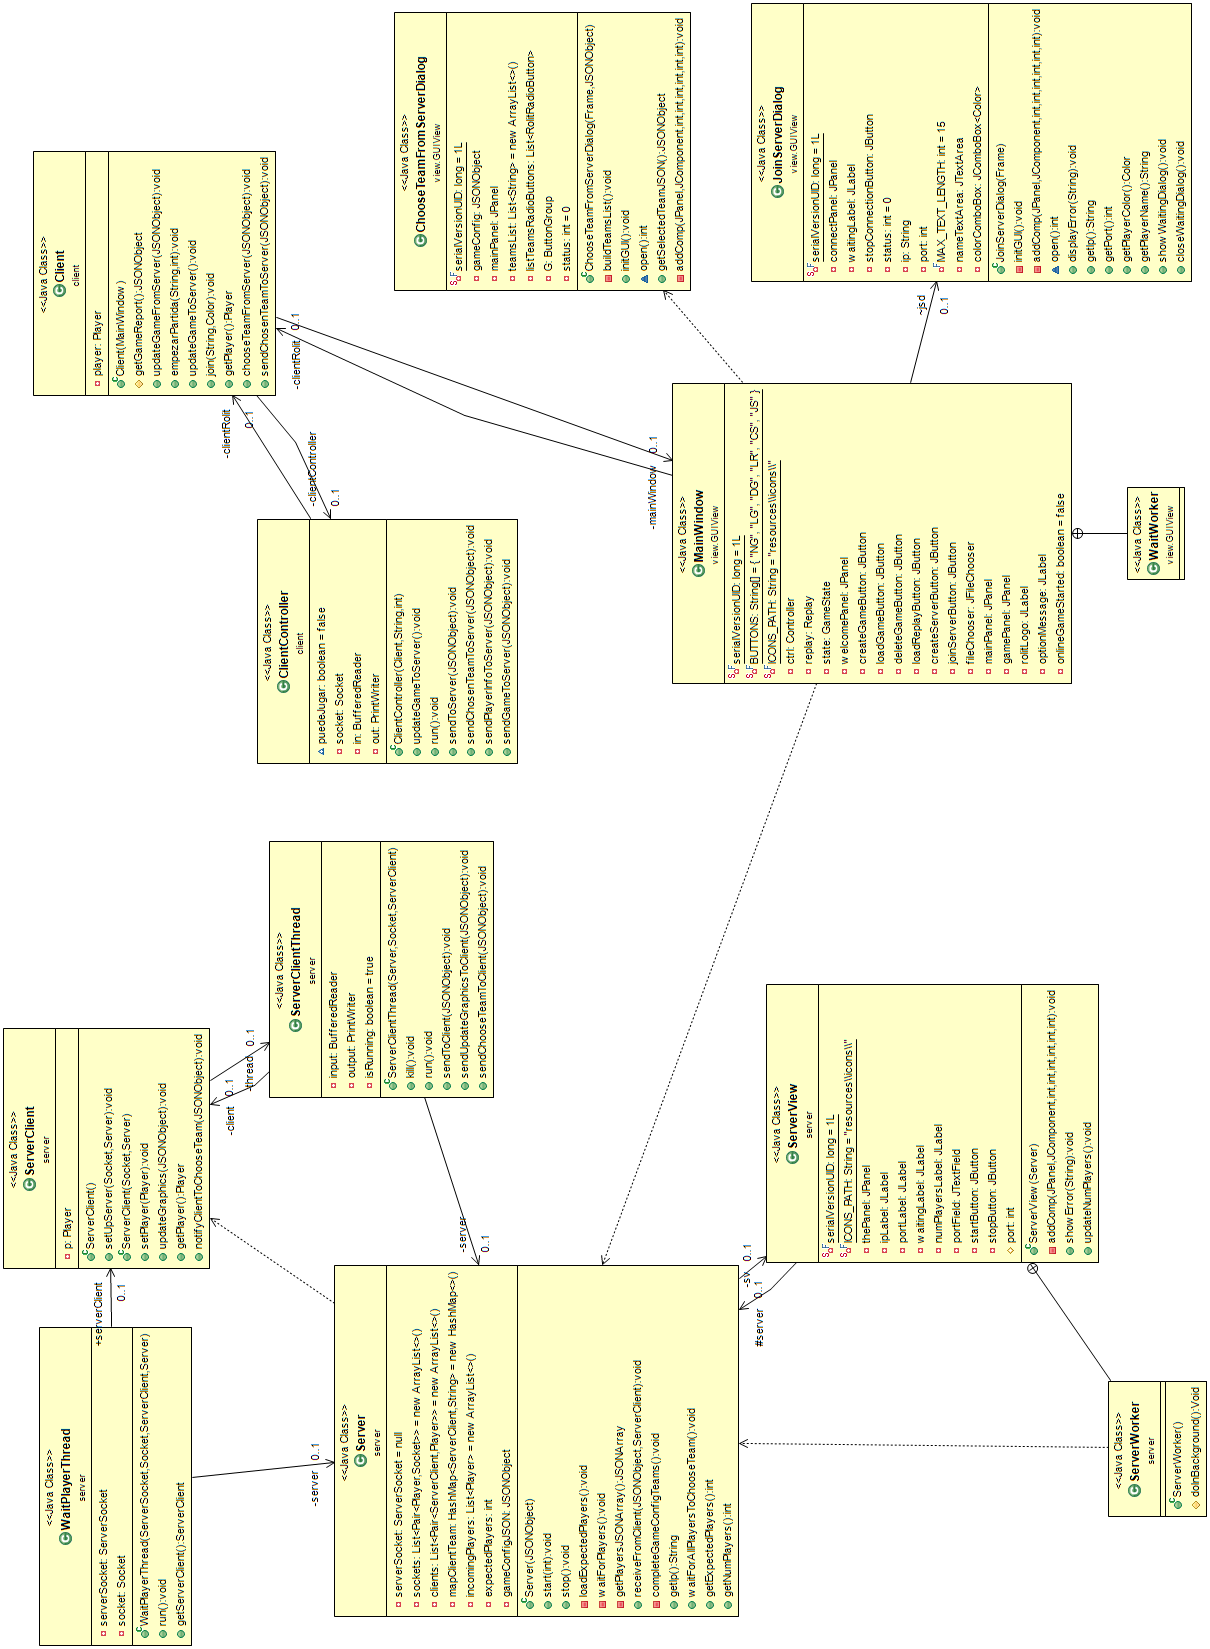
\includegraphics[scale=0.25]{UMLClasesRedSprint6.png} 
\end{center}

\end{itemize}

Por último las sucesivas refactorizaciones pugnadas desde otras partes del código (para, por ejemplo soportar la IA) precisan de un debug extensivo en el modo Red. Este debug es satisfactorio.

Los nuevos diagramas de secuencia, así como los comentarios acerca de las implementaciones de las nuevas funcionalidades se describen en el séptimo Sprint, pues en aquél se refinan ligeramente estas.

\end{sprint}
\begin{sprint}[7]

En cuanto a la red, si bien está conclusa llegados a este Sprint, el debug realizado en otras zonas del código influyen directamente en la funcionalidad de Red. Se lleva a cabo un debug rápido pero extensivo para verificar que el modo de juego en red no ha sido afectado, llevándose a cabo con éxito.

Por último, se procede a crear y solventar algunas issues relativas a la experiencia de usuario jugando en red, conllevando una serie de modificaciones que hacen más intuitiva las instrucciones para realizar la conexión.

Procedemos a comentar cómo se implementó el modo por equipos en red.

Si se escoge el modo por equipos cuando se crea una partida, el gameConfigJSON pasado como parámetro ahora adoptará la estructura de report de juego por equipos, tal y como especificamos en el documento de reports.

Dentro del método waitForPlayers que, recordemos, ejecuta un bucle de número de vueltas número de jugadores realizando las conexiones, cuando se finaliza la ejecución del bucle (es decir, cuando todos los jugadores están conectados y sus informaciones almacenadas en los atributos de Server), llama después a completeGameConfigAndSendToClients(), encargado de rellenar el gameConfig; una vez completo, se envía a los clientes.

La diferencia con anteriores sprints es que ahora el servidor, antes de completar el gameConfigJSON con la información relativa a los jugadores, comprueba en gameConfigJSON si el modo escogido es por equipos.

\begin{lstlisting}[frame=single, language=Java]
//...Bucle que realiza las conexiones con los clientes
	
if (gameConfigJSON.get("type").equals("GameTeams")) {
 for (int i = 0; i < clients.size(); ++i) {
  clients.get(i).getFirst()
  .notifyClientToChooseTeam(gameConfigJSON);
 }
			
 waitForAllPlayersToChooseTeam();
			
 completeGameConfigTeams();
			
}
	
complateGameConfigPlayers();
	
//... actualizar los clientes con el nuevo gameConfigJSON
\end{lstlisting}

De ser así, se procede a llamar a una serie de métodos cuyo fin es notificar a los usuarios para que escojan un equipo; una vez todos los usuarios han escogido equipo, se añade esta información al gameConfigJSON; posteriormente, como en la implementación de sprints anteriores, procede a completarse el gameConfigJSON con la información de los jugadores.

Primero, como observamos, se llama al método notifyClientToChooseTeam de todos los Client; este, por medio de ServerClientThread envía el gameConfigJSON, con el campo "chooseTeam" como notificación (explicaremos posteriormente cómo funcionan las notificaciones), al cliente.

Cada cliente en su respectivo ClientController recibe esta información. Observa la naturaleza de la notificación; como esta es chooseTeam, procede a abrir un diálogo ChooseTeamFromServerDialog para escoger uno de los equipos ofrecidos desde el servidor. Nótese que la información de los equipos viene proporcionada en el gameConfigJSON enviado desde el servidor.

Una vez todos los clientes han sido notificados, se llama a waitForAllPlayersToChooseTeam(). Su cometido es el de detener el hilo de ejecución hasta que todos los jugadores han escogido equipo y el servidor conoce sus elecciones.

Su implementación es la siguiente:

\begin{lstlisting}[frame=single, language=Java]
public synchronized void waitForAllPlayersToChooseTeam() {
 while ((mapClientTeam.size() != expectedPlayers)) {
  try {
   wait(500);
  } catch (InterruptedException e) {
   e.printStackTrace();
  }
 }
}
\end{lstlisting}

Como puede verse, se ha introducido como nuevo atributo del servidor un HashMap de ServerClient - Nombre del equipo escogido. Este mapa se actualiza en tiempo real conforme los clientes envían al servidor su elección de equipo. Cada medio segundo se comprueba si todos los jugadores han elegido equipo; de ser así, finaliza el método y se sigue con la ejecución de completeGameConfigAndSendToClients().

¿Cómo los clientes notifican al servidor su elección? Una vez un cliente elige equipo, manda al servidor un JSONObject con el nombre del equipo elegido en el campo "team". Antes de enviarlo, pone en el JSON un campo "notification" con el valor "chooseTeam"; para que así el servidor pueda conocer las intenciones del envío de la información por parte del cliente (notificar que se ha escogido un equipo, y cuál).

El servidor recibe un JSON con la notificación chooseTeam; en receiveFromClient (Server) observa que al ser la notificación "chooseTeam", debe añadir una nueva entrada al mapa ServerClient - Nombre del equipo escogido.

Como hemos comentado, una vez todos los equipos han sido escogidos, se sigue completando el gameConfig; ahora se sigue el mismo hilo de ejecución especificado en los anteriores sprints; se rellena el gameConfigJSON con la información de los jugadores y posteriormente se pasa el JSON a todos los clientes para que actualicen sus vistas para mostrar el juego por primera vez.

En cuanto al nuevo sistema de notificaciones, son los thread de servidor y cliente los que añaden la notificación al json a enviar; para saber qué notificación enviar, las clases en contacto con los thread (ServerClient desde el servidor, Client desde el cliente) llaman al método especifico que pondrá la notificación requerida para después enviársela al cliente/servidor.
\begin{lstlisting}[frame=single, language=Java]
//ServerClientThread.java

public void sendToClient(JSONObject json) {
 String msg = json.toString();
 if(msg != null) 
  output.println(msg);
}

public void sendUpdateGraphicsToClient(JSONObject json){
 json.put("notification", "updateGraphics");
 sendToClient(json);
}

public void sendChooseTeamToClient(JSONObject
gameConfigJSON) {
 gameConfigJSON.put("notification", "chooseTeam");
 sendToClient(gameConfigJSON);
}
\end{lstlisting}

\begin{lstlisting}[frame=single, language=Java]
//ClientController.java

public void sendToServer(JSONObject report) {
 String msg = report.toString();
 out.println(msg);
}

public void sendChosenTeamToServer(JSONObject
selectedTeamJSON) {
 selectedTeamJSON.put("notification", "chooseTeam");
 sendToServer(selectedTeamJSON);	
}

public void sendPlayerInfoToServer(JSONObject report) {
 report.put("notification", "playerInfo");
 sendToServer(report);
}
	
public void sendGameToServer(JSONObject report) {
 report.put("notification", "updateGraphics");
 sendToServer(report);
}
\end{lstlisting}

De esta forma, se tienen en cuenta las notificaciones a la hora de procesar los mensajes enviados:

\begin{lstlisting}[frame=single, language=Java]
//ClientController.java

if (newGameJSON.getString("notification")
.equals("updateGraphics"))
 clientRolit.updateGameFromServer(newGameJSON);
else if (newGameJSON.getString("notification")
.equals("chooseTeam"))
 clientRolit.chooseTeamFromServer(newGameJSON);
}
\end{lstlisting}
\begin{lstlisting}[frame=single, language=Java]
//Server.java

String notification = json.getString("notification");
		
if (notification.equals("chooseTeam")) {
 mapClientTeam.put(client, json.getString("team"));
}
else if (notification.equals("updateGraphics")) {
//...llamar a actualizar las vistas de todos los clientes...
else if (notification.equals("playerInfo")){
 Player p = new Player(json);
 incomingPlayers.add(p);	
}
\end{lstlisting}

Cambios de importancia para comparar los UML del Sprint 5 con los del Sprint 7 son los siguientes:

--En construcción--

Procedemos a actualizar los UML mostrados en el Sprint 5 para mostrar el estado final de la redes.

--En construcción--
\end{sprint}

\subsection{Como usuario quiero que Rolit introduzca características innovadoras siendo intuitivo y cómodo de jugar}
\subsubsection{Como usuario, me gustaría que se pudiese guardar y cargar partida para continuar más tarde porque permite poner en pausa el juego}
\begin{sprint}[1]
Desde el primer sprint tuvimos clara la necesidad de tener una clase que se encargase de gestionar la comunicación del programa con el exterior para cargar y guardar partidas, el \textit{SaveLoadManager}.

\begin{center}
\centering
\includegraphics[scale=0.5]{save-load-manager-sprint1.png}
\end{center}

Como se observa, inicialmente era una clase muy sencilla, pues solo tenía funciones para cargar y guardar un \textit{Game}.

\begin{center}
\centering
\includegraphics[scale=0.5]{load-sprint1.png}

Cargar partida
\end{center}

\begin{center}
\centering
\includegraphics[scale=0.5]{save-game-sprint1.png}

Guardar partida
\end{center}
\end{sprint}

\begin{sprint}[2]
En la versión anterior del \textit{SaveLoadManager}, la clase trabajaba a nivel de \textit{Game}, lo cual no tenía mucho sentido desde el punto de vista de la programación orientada objetos, pues no es necesario acceder a todos sus métodos. Por esta razón, se creo una interfaz \textit{Saveable} que debía implementar \textit{Game} para poder ser guardada y cargada de en un fichero.

\begin{center}
\centering
\includegraphics[scale=0.5]{saveable-sprint2.png}
\end{center}

\end{sprint}

\begin{sprint}[3]
Aunque el sprint 2 supuso un cambio positivo, seguía sin ser lo que buscábamos para el \textit{SaveLoadManager} en nuestro proyecto. Si bien es cierto que la interfaz \textit{Saveable} restringía los métodos de \textit{Game}, era una interfaz muy concreta y que solo se podía implementar en dicha clase.

La adquisición de nuevos conocimientos nos permitió tomar una decisión de diseño que marcaría el desarrollo de la aplicación de aquí en adelante. Desde este sprint toda la comunicación con el exterior se realizaría mediante JSONObjects.

\begin{center}
\centering
\includegraphics[scale=0.5]{reportable.png}
\end{center}

De esta forma, la interfaz \textit{Saveable} fue reemplazada por \textit{Reportable}, que se podía implementar en cualquier clase del proyecto y que contaba con un único método \textit{report()}, que devuelve una serialización del objeto en formato JSON. Además, se creo un documento en el que se especificaban todos los reports de cada clase. Puede accederse al documento actual de reports haciendo click aquí. %FIXME poner referencia al documento de los reports


\begin{center}
\centering
\includegraphics[scale=0.5]{save-load-manager-sprint3.png}
\end{center}

Esto supuso una refactorización completa del \textit{SaveLoadManager} y, aunque se mantuvo la esencia de los métodos que contenía fueron, todos fueron reimplementados completamente.

\end{sprint}

\begin{sprint}[4]
Las introducción de formas para los tableros obligó a cambiar los reports y a implementar algunos métodos extras en el \textit{SaveLoadManager} para poder mantener esta funcionalidad.
\end{sprint}

\begin{sprint}[6]
La similaridad entre los métodos para guardar partidas y \textit{replays} en el \textit{SaveLoadManager} dio lugar a una pequeña generalización de los métodos privados que permitiese reutilizarlos para guardar cualquier tipo de archivo.
\end{sprint}

\subsubsection{Como usuario, me gustaría poder guardar y cargar distintas partidas, eligiendo el nombre del fichero donde se cargan/guardan}
\begin{sprint}[2]
La refactorización llevada a cabo en el SaveLoadManager incluyó la libre elección del nombre del fichero que contiene la partida guardada, así como su ruta.

\begin{center}
\centering
\includegraphics[scale=0.5]{save-load-manager-sprint2.png}
\end{center}

\end{sprint}

\subsubsection{Como usuario, me gustaría que se pudiera guardar repeticiones de partida para poder revisarlas más tarde}
\begin{sprint}[3]
Durante el sprint 3 comenzó el desarrollo de esta funcionalidad, que de ahora en adelante denominaremos como \textit{replays}. Para su implementación, se planteó abstraer la clase Game mediante estados que representen cada uno de los momentos que atraviesa el juego a lo largo de una partida. Así, mediante un conjunto de estados es posible replicar una partida al completo.

Inicialmente se planteó que los estados almacenaran únicamente el cubo que se añade en su turno, pero esta idea fue descartada debido a que la colocación de un cubo puede llegar a afectar a cualquier parte del tablero, teniendo que incluir la lógica correspondiente para calcular los cambios. Por ello, se decidió que cada estado guardase una copia de \textit{Game} en el momento deseado.

Sin embargo, durante una \textit{replay} no se debería de poder alterar el juego, haciendo que carezca de sentido que los estados tengan acceso a  los métodos de la clase \textit{Game}, pues el único objetivo es mostrar una información inmodificable al usuario.

De esta manera surge la interfaz \textit{Replayable}, que extiende de la interfaz \textit{Reportable} y que contiene dos métodos: \textit{toString()}, para facilitar la visualización en la vista de consola, y \textit{report()}, para poder almacenar los estados en formato JSON.

\begin{center}
\includegraphics[scale=0.5]{replayable-reportable-sprint-3.png}
\end{center}

Una vez ideada esta interfaz, ya es posible definir la clase \textit{State}, que representa los estados que hemos estados describiendo hasta ahora y que, además, cuenta con el comando que la generó.

\begin{center}
\includegraphics[scale=0.5]{state-sprint-3.png}
\end{center}

El siguiente paso fue la creación de una clase contenedora de los estados, con la responsabilidad añadida de saber gestionarlos, la clase \textit{Replay}. Esta clase contiene una lista de \textit{State} que se completa durante una partida.

\begin{center}
\includegraphics[scale=0.6]{addState-replay-sprint-3.png}

Generación de lista de estados
\end{center}

Cuando la partida acaba o el usuario hace que acabe (mediante el uso del comando exit), se pregunta si desea que se guarde la repetición y se procede según su respuesta.

\begin{center}
\includegraphics[scale=0.6]{saveReplay-sprint3.png}

Guardado de Replay
\end{center}

Finalizada la generación de las \textit{replays} era el momento de hacer que pudieran cargarse y ser interpretadas para su correcta visualización. Como ya mencionamos anteriormente, la clase \textit{Replay} es la encargada de gestionar los estados y, por ello, la que contendrá esta lógica.

La función para cargar una \textit{replay} es análoga a la utilizada para guardarla y es gestionada por el \textit{SaveLoadManager}. La ejecución de una repetición comienza llamando al método \textit{startReplay()}, la clase comienza a visualizar el primer estado de su lista y entra en un bucle que permite recorrerla mediante el uso de los símbolos ``+" y ``-".

\begin{center}
\includegraphics[scale=0.7]{consola-replay-sprint-3.png}
\end{center}

Con estas repeticiones de partidas funcionales dimos por completada esta tarea en el Sprint 3.
\end{sprint}

\begin{sprint}[4]

Este sprint se caracterizó por la implementación de una GUI funcional, lo que conlleva la adaptación de las \textit{replays} a este nuevo formato. Decidimos que la comunicación entre modelo y vista se llevara a cabo mediante el uso del patrón observador, lo cual supuso un reto inicial para las repeticiones de partidas.

Basta detenerse a pensar unos minutos para darse cuenta que, cuando cargamos, procesamos y visualizamos una \textit{replay} desde un fichero, la clase \textit{Game} no interviene en el proceso, pues es la clase \textit{Replay} la encargada de gestionar toda la lógica de las repeticiones. Por tanto, la clase \textit{Replay} es también un modelo que debe ser observado.

\begin{center}
\includegraphics[scale=0.5]{rolit-observer-sprint4.png}
\end{center}

Para implementar los observadores se creó la interfaz \textit{ReplayObserver} que tiene métodos para notificar cuando se avanza a la izquieda, a la derecha y para mostrar mensajes en la barra de estado. Además, se añadieron algunos getters necesarios a las clases \textit{Replay} y \textit{State}.

\begin{center}
\includegraphics[scale=0.5]{replay-state-sprint-4.png}
\end{center}

\end{sprint}

\begin{sprint}[5]
La GUI sufrió una refactorización, siendo necesario para ello la creación nuevos getters. Además, la refactorización  de la clase \textit{Controller} trajo consigo problemas con las \textit{replays} que no serían solucionados en este sprint por falta de tiempo.
\end{sprint}

\begin{sprint}[6]
El cambio de paradigma en el funcionamiento mediante la introducción de su propio hilo y el nuevo controlador del sprint anterior hicieron que fuese necesario modificar cómo se guardan los estados en la clase \textit{Replay}.

Además, la necesidad de notificar a la vista con el Replay para que sea guardada en caso de que así lo desee el usuario, tiene como consecuencia que la clase \textit{Game} sea la encargada de generar sus propias repeticiones. Este proceso puede verse reflejado en el siguiente diagrama de secuencias.
\begin{center}
\includegraphics[scale=0.5]{addState-replay-sprint-6.png}
\end{center}

\end{sprint}

\subsubsection{Como usuario, me gustaría poder salir del juego en cualquier momento}
\begin{sprint}[2]
Con la introducción de los comandos vino acompañado el comando exit, que puede ser ejecutado en cualquier momento durante la partida para detener la ejecución del juego.

\begin{center}
\includegraphics[scale=0.5]{exit-sprint2.png}
\end{center}

En sprints posteriores este diagrama dejará de ser válido debido a refactorizaciones en el controlador, aunque la clase ExitCommand ha permanecido invariante. Los cambios sufridos para este comando son análogos a los del resto, que pueden ser consultados en ... %FIXME Poner donde esté explicada la evolución de los comandos y una referencia a esa seccion
\end{sprint}

\end{document}